\documentclass[a4paper, 12pt, french, twoside]{article}
\usepackage{graphicx,wrapfig,lipsum}
\usepackage{graphicx}
\usepackage{mathtools}
\usepackage{amsmath}
%\frenchbsetup{StandardLists=true} à inclure si on utilise 
\usepackage[french]{babel}
\usepackage{enumitem}
\usepackage{float}
%\usepackage[top=2.5cm, bottom=2cm, left=2cm, right=2cm, showframe]{geometry}
\usepackage[top=2.5cm, bottom=2cm, left=2cm, right=2cm]{geometry}
\usepackage{caption}
\usepackage{amsmath}
\usepackage{graphicx} % Required for inserting images
\usepackage{subcaption}
\usepackage{hyperref}
\usepackage{makecell}
\usepackage{amsfonts}
\usepackage{amsthm}


\newtheorem{theorem}{Théorème}[section]
\newtheorem{corollary}[theorem]{Corollaire}
\newtheorem{lemma}[theorem]{Lemme}
\newtheorem{proposition}[theorem]{Proposition}
\newtheorem{defi}[theorem]{Définition}
\newtheorem{rem}[theorem]{Remarque}

\usepackage{pdfpages} % lien Pdf test
 \usepackage{tcolorbox}

\usepackage{cleveref}
\crefrangelabelformat{equation}{(#3#1#4--#5#2#6)}
\crefname{equation}{Eq.}{Eqs.}
\Crefname{equation}{Equation}{Equations}


%\usepackage{movie15}
\usepackage{epstopdf}
\usepackage{subcaption}
\usepackage{multicol}

%a abréviations
\def \be {\begin{equation}}
\def \ee {\end{equation}}
\def \dd  {{\rm d}}
\def \bm {\begin{pmatrix}}
\def \em {\end{pmatrix}}

%Ensembles 
\newcommand{\Cc}{{\mathbb{C}}}
\newcommand{\Ct}{\Cc^\times}
\newcommand{\Hh}{{\mathbb{H}}}
\newcommand{\Nn}{{\mathbb{N}}}
\newcommand{\Zz}{{\mathbb{Z}}}
\newcommand{\Zzn}{\Zz/n\Zz}
\newcommand{\ZzNt}{(\Zz/N\Zz)^\times}%quotient 
\newcommand{\Rr}{{\mathbb{R}}}
\newcommand{\Rt}{{\Rr^\times}}
\newcommand{\Qt}{{\Qq^\times}}
\newcommand{\Qq}{{\mathbb{Q}}}
%to do later
\newcommand{\later}[1]{\textcolor{orange}{[#1]}}
\newcommand{\com}[1]{\textcolor{magenta}{[#1]}}

%to make hyper refs not surrounded with red
\hypersetup{pdfborder=0 0 0}
\hypersetup{
    colorlinks=true,
    linkcolor=blue,
    filecolor=magenta,      
    urlcolor=cyan,
    pdftitle={Overleaf Example},
    pdfpagemode=FullScreen,
    }
    
\title{Document speaker 1}

\begin{document}

\maketitle


\section{Remerciements + buts du poly} 

\textbf{Peu de preuves à l'oral, dire qu'elles sont dans le cours et bosser l'intuition++ poly hyper dense destiné à accompagner le premier semestre. Tout ne sera pas vu dans le cours, prendre son temps no pressure.}

\subsection{Qu'est-ce que l'analyse}

L'analyse est l'étude de l'infinitésimal. Cette branche des mathématiques traite de limites, de continuité, de dérivé et d'intégration. En fait, on tous fait de l'analyse au lycée ou au gymnase parce qu'étudier les fonctions en fait partie! De plus, les notions de limite et d'infinitésimal ont déjà été vue. Il suffit de se rappeler la définition de la dérivée d'une fonction.

Donc, nous allons étudier cette branche des mathématiques. Pour se faire, nous allons commencer par étudier les suites puis les séries et les fonctions. Les suites seront essentielles à la démonstration de plusieurs propriétées des fonctions. Quelques concepts dans ce cours seront vu plus en détails en algèbre linéaire tel que les notions sur les ensembles. Finalement, plusieurs parties écrites ne sont présentées que pour satisfaire la curiosité du lecteur et ne sont pas obligatoires pour cette première approche de l'analyse ou encore pour ce premier semestre. 




\subsection{Différents types de démonstrations}

Lorsque que l'on cherche à démontrer une proposition, il se peut que l'on ne sache comment commencer. C'est pourquoi connaître les différents types de démonstrations peut aider. Nous allons donc procéder à une énumération de plusieurs techniques!


\subsubsection{Preuve directe}
Premièrement, il y a la preuve directe. Celle-ci consiste à prouver de façon directe la proposition. 
\subsubsection{Preuve par contraposition}
Puis, il existe la preuve par contraposition. Celle-ci se base sur le fait que si A implique B, alors non B implique non A. Si être français implique être européen, alors ne pas être européen implique ne pas être français. Il faut noter que B n'implique pas forcément A car être européen n'implique pas forcément français.


\subsubsection{Preuve par l'absurde}
De plus, il existe le raisonnement par l'absurde. Celui-ci consiste à supposer que la conclusion de la proposition est fausse et montrer que ce n'est pas cohérent.

\subsubsection{Preuve par récurrence}
Il existe aussi le raisonnement par récurrence qui sera utilisé dans le contexte des suites. Il sert à démontrer une propriété valable pour tous les entiers naturels. Cela consiste en trois étapes: l'initialisation montre que la propriété est valable pour le premier terme, $x_0$ par exemple, la récurrence montre que si c'est valable pour le terme $x_n$ alors c'est valable pour le terme $x_{n+1}$, puis la conclusion permet de conclure que la propriété est valable pour tous les termes. Il suffit de prendre l'analogie de l'échelle: si on sait qu'on peut monter sur le premier barreau et que si on est sur n'importe lequel, on peut monter sur celui d'après, alors on peut aller sur n'importe quel barreau! 

\subsection{Vocabulaire mathématique (A mettre sur une slide !)}

Les mathématiques ont un langage particulier: des symboles permettent d'énoncer des conditions beaucoup plus vite. Ces symboles peuvent parfois être complexes à comprendre lorsqu'ils s'assemblent entre eux. Nous allons donc revoir le sens de chacun et des exemples de "phrases" composées grâce à ceux-ci.



\begin{center}
\begin{tabular}{|m{1.5cm} |m{8cm}| m{6.5cm}|} 
 \hline
 Symbole & Signification & Exemples\\ [0.5ex] 
 \hline
 = & Egalité entre les deux côtés & $a=5$: $a$ prend la valeur 5.  \\ 
 \hline
 $\doteq$ ; := & est défini par & $f(x)\doteq x^2$: on définit la fonction $f$ par la fonction $x^2$.  \\
 \hline
 $\implies$ & Implique & Avoir des cheveux bruns $\implies$ Avoir des cheveux \\
 \hline
 $\iff$ & Est équivalent & Avoir des cheveux $\iff$ Ne pas être chauve\\
 \hline
 \{...\} & Définition d'un ensemble discret & $\Nn$=\{1, 2, 3, ...\}  \\
 \hline
 [...] & Définition d'un intervalle continu fermé, ie, les bornes sont contenues dans l'intervalle & [0,1]  \\
 \hline
 ]...[ ; (...)& Définition d'un intervalle continu ouvert, ie, les bornes ne sont pas contenues dans l'intervalle. (On peut choisir de n'ouvrir qu'une seule borne) & ]0,1[  \\
 \hline
  $\in$ & Appartient à & 2 $\in$ {1, 2, 3} \\
 \hline
 $\notin$ & N'appartient pas à & 4 $\notin$ {1, 2, 3} \\
 \hline
 
 $\backslash$ & Privé de & {1, 2, 3}={1, 2, 3, 4}\ {4} \\
 \hline
 $\forall $ & Pour tous & $f(x)\doteq x^2, \forall x\in \Rr$\\
 \hline
 \end{tabular}
 \end{center}
 \begin{center}
\begin{tabular}{|m{1.5cm} |m{8cm}| m{6.5cm}|} 
 \hline
 $\exists$ & Il existe  & $\exists x \in \Zz $ tel que $x^2=1$, $x=1$ ou $x=-1$\\
 \hline
 $\exists !$ & Il existe un unique & $\exists ! x \in \Nn$ tel que $x^2=1$, $x=1$ \\
 \hline
 ;& Avec & $\Nn=\{q\in \Zz ;  0\leq q\}$, l'ensemble des entiers positifs est constitué de l'ensemble des entiers avec comme condition qu'ils soient positifs.\\
 \hline
 \end{tabular}
\end{center}

Ce dernier exemple a mis en évidence les phrases que l'on peut créer. Après un ';', on peut mettre le nombre de conditions que l'on souhaite, tant qu'elles sont cohérentes. 

Lorsque l'on traite d'une application ou plus spécifiquement d'une fonction, on peut la noter de la façon suivante :

\begin{equation}
    f: A \to B,
\end{equation}
ce qui signifie que $f$ est une application qui a comme ensemble de départ $A$ et comme ensemble d'arrivée $B$. Donc elle prend des éléments de $A$ et attribue à chacun un élément de $B$. La théorie des applications sera vue en algèbre. Nous traiterons des fonctions dans ce polycopié, mais des fonctions réelles donc qui ont pour valeurs des réels. Ainsi, on a $B=\Rr$.\\

Un dernier symbole souvent utilisé est $\Box$. Il intervient dans la rédaction de preuve. Celles-ci peuvent se finir avec ce symbole, ce symbole mais colorié en noir, avec "CQFD",... Bref, trouvez votre moyen de les finir mais le $\Box$ sera utilisé dans ce polycopié.

\subsection{Rappels trigonométriques}

Les fonctions trigos seront utilisées dans ce cours. Un des gros avantages est quelles sont périodiques donc assez intéressantes. Il y a un rappel dans le poly que vous pouvez lire !


% Les fameuses fonctions trigonométriques sont très utiles car elles possèdent des propriétées merveilleuses pour l'analyse. Faisons un rappel de ces fonctions et de certaines identitées particulières. 

% Donc, il existe le cosinus, le sinus et la tangente. Ces fonctions sont représentées sur la figure suivantes.

% \begin{figure}[H]
%     \centering
%     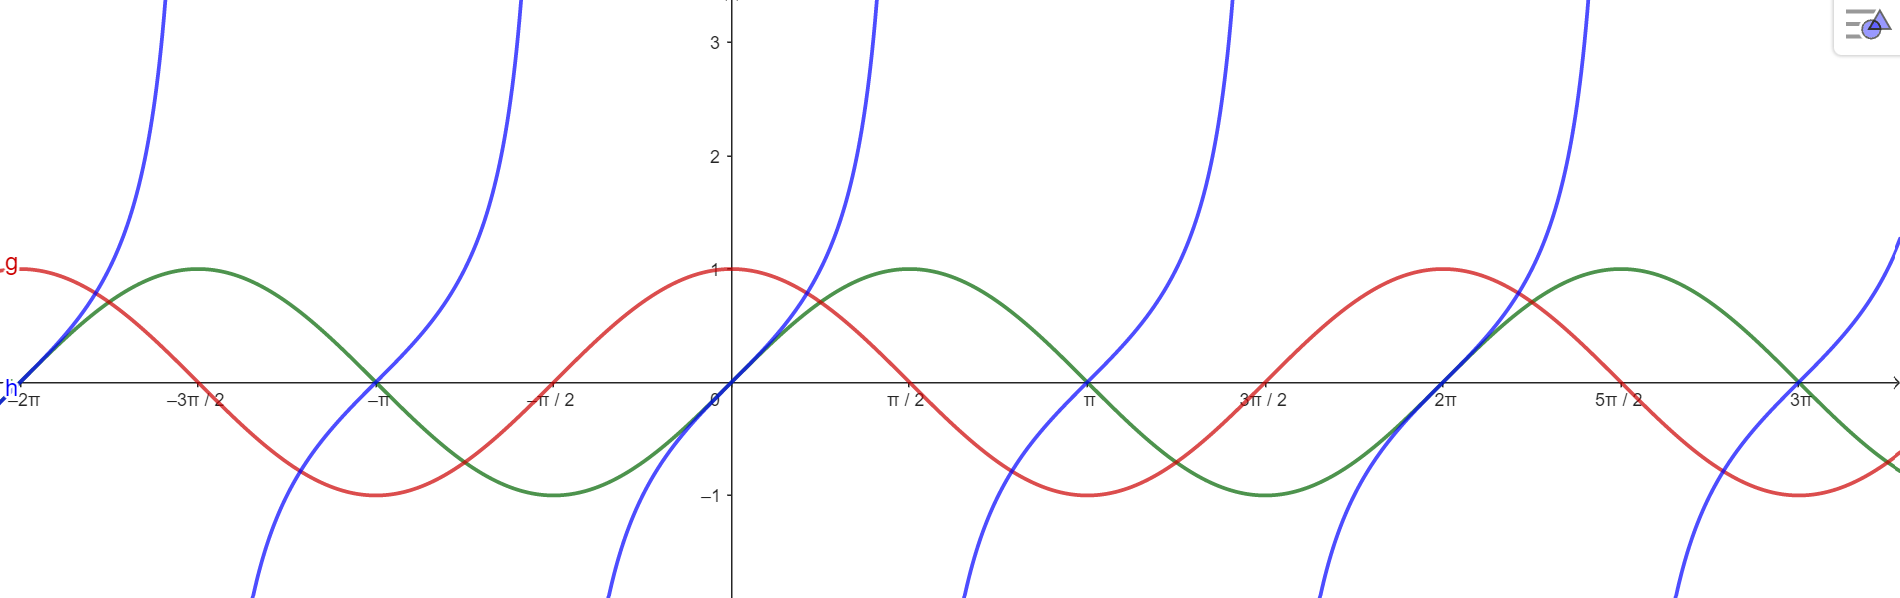
\includegraphics[scale=0.5]{Cours/trigo.png}
%     \caption{En rouge la fonction $\cos(x)$, en vert la fonction $\sin(x)$ et en bleu $\tan(x)$.}
%     \label{fig:enter-label}
% \end{figure}
% Ce que l'on observe est que chaque fonction est périodique. De plus, comme $\tan(x)=\frac{\sin(x)}{\cos(x)}$, elle est aussi périodique mais n'est pas définie en tout point: le cosinus s'annule souvent!
% Voici la relation majeure:

% \begin{equation}
%     \cos^2(x)+\sin^2(x)=1.
% \end{equation}
% Elles ont chacune des valeurs particulières qu'il est utile de connaître par coeur. Elles sont écrites dans le tableau suivant:

% \begin{center}
% \begin{tabular}{|m{1.5cm} |m{2cm}| m{2cm}|m{2cm}|} 
%  \hline
%     $\theta$ [rad] & $\cos (\theta)$& $\sin (\theta)& $\tan (\theta)\\
%     \hline
%     0& 1& 0&1\\
%     $\pi/6$ & $\frac{\sqrt{3}}{2}$ &$\frac{1}{2}$&$\frac{1}{\sqrt{3}}$\\ 
%     $\pi/4$ &$\frac{1}{\sqrt{2}}$&$\frac{1}{\sqrt{2}}$&1\\
%     $\pi/3$ &$\frac{1}{2}$& $\frac{\sqrt{3}}{2}$&$\sqrt{3}$\\
%     $\pi/2$ &0&1& Non définie\\
%     $\pi$&-1&0&0\\
%  \hline
%  \end{tabular}
% \end{center}
% notez que les angles sont donnés en radian donc en un multiple de $\pi$. Ce sera l'unité des angles dans la majorité de vos études. De plus, la relation entre degrées et angle est $\theta \text{[rad]}= \Theta\text{[deg]}\cdot \dfrac{\pi}{180}$.




\section{Chap 1}
\subsection{Les ensembles}
Commençons par quelques rappels sur les ensembles :
\begin{defi}
  Un ensemble est une collection d'objets appelés éléments de cet ensemble.   
\end{defi}
On peut avoir les ensembles suivants : 
\begin{enumerate}
    \item $E=\{\text{bleu, rouge, jaune}\}$. C'est un ensemble fini à trois éléments qui sont rouge, bleu et jaune. 
    \item $E=\{\text{toutes les couleurs}\}$. Cet ensemble est infini et ses éléments sont toutes les couleurs possibles. 
    \item $E=\{1,2,3\}$. C'est un ensemble fini de nombres. 
    \item $E=\Nn$ les entiers naturels qui seront définis plus bas. 
\end{enumerate}
Et il en existe bien d'autres, mais ceux qui vont nous intéresser en particulier sont les sous-ensembles des réels. Finissons de parler des ensembles en rappelant quelques propriétés et opérations sur les ensembles : 
\begin{enumerate}
    \item Si $x$ est un élément d'un ensemble $E$, on note $x\in E$.
    \item Si $x$ n'est pas un élément d'un ensemble $E$, on note $x\notin E$.
    \item Soit $A$ et $B$ deux ensembles, on dit que $A$ est contenu dans $B$ si tous les éléments de $A$ appartiennent aussi à $B$, on note $A\subset B$ et on dit que $A$ est un sous-ensemble de $B$. De manière équivalente, on a que $A\subset B$ si et seulement si $\forall x\in A, x\in B$.
    \item Si A$\subset B$ et $B\subset A$ alors $A=B$. 
    \item Pour $A$ et $B$ deux ensembles, on a les opérations suivantes :
    \begin{itemize}
        \item (\textit{Union}) $A\cup B=\{x; x\in A \text{ ou } x\in B\}$. 
        \item (\textit{Intersection}) $A\cap B=\{x; x\in A \text{ et } x\in B\}$. 
    \end{itemize}
\end{enumerate}
Par exemple, si on prend $A=\{1,2,3\}$, $B=\{1,2,4\}$ et $C=\{1,2,3,4\}$ on obtient :
\begin{enumerate}
    \item $A\cup B=\{1,2,3,4\}$.
    \item $A\cap B=\{1,2\}$.
\end{enumerate}
On définit aussi l'ensemble vide $\empty$ comme l'ensemble ne contenant aucun élément. Ainsi l'ensemble vide est un sous-ensemble de n'importe quel ensemble.\\\\
La théorie des ensembles est un sujet d'étude à elle seule, mais pour le moment cela nous suffira pour comprendre la suite!


\subsection{Les réels}
On a tous l'habitude d'utiliser les nombres réels, pour résoudre des équations, pour définir des fonctions, etc. Mais est-ce qu'on s'est déjà demandé s'ils existaient vraiment ? S'ils sont bien "réels" ? Alors évidemment la réponse est oui, mais comment peut-on construire cet ensemble rempli de nombres compliqués comme $\pi$ ou bien $\sqrt{2}$ ? Ce serait un peu trop ambitieux de s'essayer à construire rigoureusement les nombres réels, ici, nous allons simplement essayer de mieux comprendre cet ensemble de nombres si pratique et donner quelques propriétés de celui-ci. Commençons par les entiers naturels, c'est-à-dire les entiers positifs. 
\begin{defi} L'ensemble des entiers naturels est l'ensemble $\Nn=\{0,1,2,...\}$. 
\end{defi}

On peut bien sûr multiplier et additionner les entiers positifs entre eux, et on peut aussi définir une relation d'ordre. C'est-à-dire qu'en prenants deux entiers $n,m\in \Nn$ on peut les comparer et dire que $n\leq m $. En effet, lorsque l'on observe $2$ et $6$ ou $12$ et $5421$ on peut directement trouver lequel est "le plus grand".
% La relation "le plus grand" est une relation d'ordre qui respecte les propriétés (axiomes) suivantes : 
% \begin{enumerate} [label=\arabic*)]
%     \item \textit{(réflexivité)} pour tout $ n\in \Nn$ on a $n\leq n$.
%     \item \textit{(antisymétrie)} si pour $n,m\in \Nn$ on a $n\leq m$ et $m\leq n$ alors $n=m$.
%     \item \textit{(transitivité)} si pour $p,n,m \in \Nn$ on a $n\leq m$ et $m\leq p$ alors $n\leq p$.
%     \item \textit{(ordre total)} pour tout $n,m\in \Nn$ soit $n\leq m$ soit $m\leq n$.
% \end{enumerate}
On note aussi $\Nn^*$ les entiers strictement positifs (on enlève 0).\\\\
On peut maintenant facilement construire l'ensemble des entiers relatifs : 
\begin{defi}
    L'ensemble des entiers relatifs est l'ensemble $\Zz=\{...,-1,0,1,...\}$.
\end{defi}
Ainsi $\Zz$ "contient" $\Nn$, en effet chaque entier positif appartient aux entiers relatifs, donc on a $\Nn \subset \Zz$. On peut étendre la relation d'ordre de $\Nn$ à $\Zz$.\\\\
% Avec ces deux ensemble, on peut construire les nombres rationnels, on donne juste l'idée de la construction pour les intéressés, autrement, vous pouvez passer cette partie et allez à la partie sur la densité de $\Qq$ dans $\Rr$.
% \begin{tcolorbox}
%    \begin{defi}
%     L'ensemble des nombres rationnels est l'ensemble $\Qq=\{p/q; p,q\in \Zz; q\neq 0 \}$ muni de la relation d'équivalence suivante: 
%     $a/b\sim p/q \iff \exists n\in \Zz \text{ tq } an=p \text{ et } bn=q$
% \end{defi}
% Vous verrez ce qu'est une relation d'équivalence dans le cours d'algèbre linéaire, mais dans notre cas cette relation signifie simplement qu'une fraction "équivaut" à son unique forme réduite. Grâce a cette construction, on peut démontrer que les axiomes sont respecté et que $\Qq$ est unique. 
% \end{tcolorbox}


% La relation d'ordre étendue à $\Qq$ à en plus les deux propriétés suivantes $\forall a,b \in \Qq$:  
% \begin{enumerate}[label=\arabic*),resume]
%     \item  Si $a\leq b$ alors $\forall x\in \Qq$ on a $a+x\leq b+x$.
%     \item Si $a\leq b$ alors $\forall x\in \Qq, x\geq 0 $ on a $ax\leq bx$.
% \end{enumerate}
% On remarque que la relation d'ordre sur $\Qq$ n'est pas si bien définie, comment comparer $\frac{6}{14}$ et $\frac{2}{3}$, en effet, on pourrait dire que $\frac{2}{3}\leq \frac{6}{14} $ car $2\leq 6$ et $3\leq 14$ mais on sait bien qu'en réalité $\frac{6}{14}=\frac{3}{7}\leq \frac{2}{3}$. Ainsi pour clarifier, on définit la relation d'ordre sûr $\Qq$ comme ceci :
% \begin{center}
%     $\forall \frac{p}{q}, \frac{p'}{q'}\in \Qq$ on a que $\frac{p}{q}\leq \frac{p'}{q'}$ si et seulement si $\frac{p}{q}- \frac{p'}{q'}=\frac{pq'-p'q}{qq'}\leq 0$.
% \end{center}

% Maintenant, une question se pose: Peut-on construire les réels à partir de $\Qq$? \\\\
% On définira d'abords les nombres réels $\Rr$ de manière intuitive comme une droite munie des opérations arithmétique et d'une relation d'ordre respectant les axiomes suivants : Pour $x,y,z\in \Rr$
%     \begin{enumerate}
%         \item (\textit{associativité du +}) $(x+y)+z=x+(y+z)$.
%         \item (\textit{commutativité du +}) $x+y=y+x$.
%         \item (\textit{élément neutre du +}) $x+0=x$.
%         \item (\textit{inverse du +})$\forall x\in \Rr , \exists ! k \in \Rr$ tel que $x+k=0$, on dit que $k$ est l'inverse de $x$ et on note $k=-x$.
%         \item (\textit{associativité du $\cdot$}) $(xy)z=x(yz)$.
%         \item (\textit{commutativité du $\cdot$}) $xy=yx$.
%         \item (\textit{élément neutre du $\cdot$} $x\cdot 1=x$.
%         \item (\textit{inverse du $\cdot$} $\forall x\in \Rr , \exists ! k \in \Rr$ tel que $xk=1$, on dit que $k$ est l'inverse de $x$ et on note $k=x^{-1}$.
%         \item (\textit{distributivité}) $x(y+z)=xy+xz$
%         \item (\textit{Ordre total}) 
%         \begin{enumerate}
%             \item $x\leq y \leq z$ implique $x\leq z $.
%             \item $x\leq y$ et $y\leq x$ impliquent $x=y$.  
%             \item $\forall x,y \in \Rr$ on a soit $x\leq y$ soit $y\leq x$. 
%         \end{enumerate}
%         \item Si on a $x\leq z$ alors on aura aussi $x+z\leq y+z$.
%         \item Si $0\leq x$ et $0\leq y$ alors $0\leq xy$
%         \end{enumerate}
% Idées exos: 
% \begin{itemize}
%     \item $x\leq y$ alors $-x\leq -y$
%     \item $x\leq 0$ et $y\leq 0$ alors $0\leq xy$
%     \item $x\leq y $ et $0\leq z$ alors $xz\leq yz$
%      \item $x\leq y $ et $0\geq z$ alors $xz\geq yz$
%      \item unicité du 0 et de l'inverse 
%      \item $x\cdot 0=0$. 
% \end{itemize}
% Ainsi $\Rr$ est un corps commutatif (notion qui sera définie dans le cours d'algèbre linéaire) ordonné contenant $\Qq$, mais les réels sont beaucoup plus nombreux que les rationnels, on démontrera que $\Qq$ est "dense" dans $\Rr$. 

\subsection{Densité de $\Qq$ dans $\Rr$}
Commençons par donner un exemple d'un réel qui n'est pas un rationnel, c'est-à-dire un irrationnel: 
\begin{proposition}
    $\sqrt{2}$ n'est pas un rationnel. 
\end{proposition}
\textit{Sauter la preuve?}
\begin{proof}
   Supposons par l'absurde qu'il existe $x\in \Rr$ tel que $x^2=2$ et $x=a/b$ avec $a,b \in \Zz$. On suppose que $a/b$ et une fraction réduite, c'est-à-dire que $b\neq 0$ et que $a$ et $b$ sont premiers entre eux, donc notamment $a$ et $b$ ne sont pas tous les deux pairs. 
   $$x^2=2 \Rightarrow a^2/b^2=2 \Rightarrow a^2=2b^2$$
   Donc $a^2$ est pair, ce qui implique que $a$ est pair, donc $\exists n \in \Nn$ tel que $a=2n$. On obtient donc $$a^2=4n^2=2b^2 \Rightarrow 2n^2=b^2$$
   Ainsi $b$ est aussi pair, ce qui est impossible, car on a supposé la fraction réduite. 
\end{proof}
On vient de montrer que $\Rr \neq \Qq$!\\
Maintenant, introduisons un peu de terminologie : 
\begin{defi}
    Soit $A$ une partie de $\Rr$ (un sous-ensemble), on dit que : 
    \begin{enumerate}
        \item $A$ possède une borne supérieure (est majoré) si $\exists b \in \Rr $ tel que $\forall a \in A$ on a $a\leq b$. On dit alors que $b$ est un majorant de $A$. 
        \item $A$ possède une borne inférieure (est minoré) si $\exists b \in \Rr $ tel que $\forall a \in A$ on a $a\geq b$. On dit alors que $b$ est un minorant de $A$. 
    \end{enumerate}   
\end{defi}
\begin{defi}
    
\textbf{(Axiome de complétude)}  Pour toute partie $A$ de $\Rr$ majorée, il existe un $s\in \Rr$ tel que: 
\begin{itemize}
    \item $s$ est un majorant pour $A$.
    \item $\forall b$ majorant de $A$, on a $s\leq b$.
\end{itemize}
C'est-à-dire que $s$ est la plus petite des bornes de $A$.
\end{defi}
\begin{defi}
    Ce $s$ est unique et est appelé le suprémum de $A$, noté sup$(A)$.  
\end{defi}
\begin{rem}
    De même pour une partie $A$ minorée, il existe un $i\in \Rr$ tel que :
    \begin{itemize}
    \item $i$ est un minorant pour $A$
    \item$\forall b$ minorant de $A$, on a $i\geq b$
\end{itemize}
    Dans ce cas cet unique $i$ est appelé l'infimum de $A$, noté inf$(A)$.
\end{rem}
\begin{rem}
    Si $s=$sup$(A)$ est tel que $s\in A$ alors dans ce cas on peut dire que $s$ est un maximum, de même pour $i$ qui sera un minimum.  
\end{rem}
Pour mieux comprendre ces définitions très abstraites, voici quelques exemples: 
\begin{enumerate}
\item $\Nn$ est minoré, mais pas majoré. 
\item $\Rr$ n'est ni minoré ni majoré. 
\item $(a,b)$ est minoré et majoré. 
    \item Pour $A=[0,1[$, on a sup$(A)=1=s$ et inf$(A)=0=i$ avec $s$ qui n'est pas un maximum et $i$ qui est un minimum. 
\end{enumerate}
La suite est en "bonus" et elle sera couverte en cours durant l'année, ci cela vous semble trop dur pour le moment vous pouvez sauter la partie suite.
% \begin{tcolorbox}
    

% Afin de prouver la densité de $\Qq$ dans $\Rr$, nous avons besoin de la propriété suivante: 
% \begin{proposition}
%     (\textit{Propriété archimédienne})\\
%     Soient $x,y\in \Rr$ avec $x>0$. Alors, il existe un $n\in \Nn^*$ entier tel que:
%     $$nx>y$$
% \end{proposition}
% \begin{proof}
%     On considère l'ensemble $A={nx;n\in \Nn^*}$. Si on suppose par l'absurde que $y$ est un majorant de $A$, c'est-à-dire $\forall z\in A$ $z\leq y $ ou bien $\forall n\in \Nn^*$ $nx\leq y $. Alors $A$ est majoré donc par l'axiome de complétude, $\exists s$ un suprémum de $A$. \\
%     Puisque $x>0\Rightarrow s-x<s$ donc $s-x$ n'est pas un majorant de $A$ par définition du suprémum. Donc $\exists m \in \Nn^*$ tel que $s-x<mx$ mais alors $s<x(m+1)\in A$ d'ou la contradiction car $s$ est le suprémum de $A$. donc $A$ n'est pas majoré par $y$ donc on peut trouver un $nx\in A$ tel que $nx>y$. 
% \end{proof}


    

% \begin{theorem}
%    $\Qq$ est dense dans $\Rr$, c'est a dire que $\forall x<y \in \Rr$, $\exists q\in \Qq$ tel que $x<q<y$.  
% \end{theorem}

Donc la densité peut se voir comme le fait qu'entre deux nombres irrationnels, aussi proche soient-ils, on pourra toujours trouver un nombre rationnel. L'espace est vraiment continu donc il n'y aucun trou sur la droite des réels. 

% \begin{proof}
%     Comme $x<y$ on a $y-x>0$ donc par la propriété d'Archimède, on trouve $q\in \Nn^*$ tel que $q(y-x)>1 \Rightarrow q>\frac{1}{y-x}\Rightarrow qy-qx>1$. 
%     \begin{enumerate}
%         \item Si $qy\notin \Zz$ alors la propriété archimédienne nous dit que l'ensemble $\{n\in \Zz; n>qy\}$ est minoré, non vide, alors on prend $i$ son infimum et on pose $p=i-1$, alors $p<qy$ et $qx<p$ car $qy-qx>1$. 
%         \item Si $qy\in \Zz$ alors on pose $p=qy-1$ et on a bien $qx<p<qy$. 
%     \end{enumerate}
%     Donc dans tout les cas, un tel $p$ existe. Cela nous donne $p/q \in \Qq$ tel que: 
%     $$x<p/q<y.$$
% \end{proof}


% \end{tcolorbox}
%  On peut aussi démontrer que l'ensemble $\Rr \backslash \Qq$ des irrationnels est aussi dense dans $\Rr$.Le fait que $\Qq$ soit dense dans $\Rr$ implique que dans n'importe quel intervalle ouvert non vide de $\Rr$, il y a une infinité de rationnels et d'irrationnels. Cela veut aussi dire que chaque nombre irrationnel peut être approximé par un nombre rationnel. Ce résultat est un résultat très important, notamment pour mieux comprendre le concept de continuité qui sera défini plus tard. 
\newpage
\section{Chap 2}
Dans ce chapitre, nous allons aborder le concept de suites, fondamental en analyse. Une suite est une infinité de termes, qu'on associe a des entiers naturels pour les "numéroter". Mais pour introduire les propriétés de tels objets mathématiques on doit d'abord introduire un moyen de les comprendre, la valeur absolue en lien avec la mesure d'un ensemble.
\subsection{Valeur absolue }
\begin{defi}
    La valeur absolue est un outil souvent présente en Analyse, et elle est définie comme suit.
\end{defi} 


\begin{equation}
|x|=
    \begin{cases}
        -x &{\rm si \,\, } x < 0 ,\\
        x &{\rm si \,\, } x \geq 0,
    \end{cases}
\end{equation}
\begin{figure}[H]
    \centering
    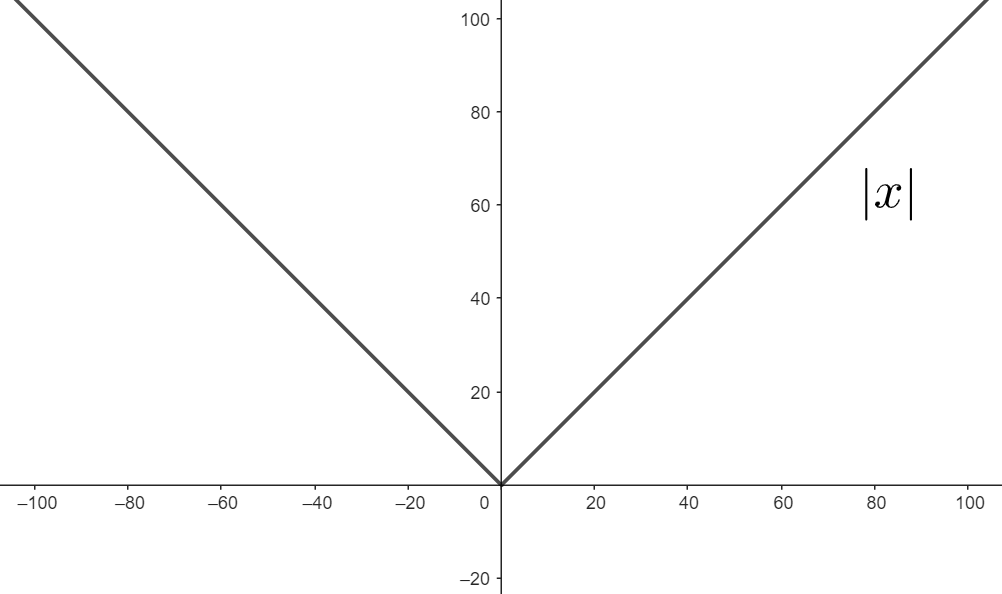
\includegraphics[scale=0.6]{Cours/vabs.png}
    \caption{Fonction valeur absolue.}
    \label{fig:enter-label}
\end{figure}

% Sa dérivée est la fonction signe et est définie comme:
% \begin{equation}
% {\rm sgn}(x)=
%     \begin{cases}
%         -1 &{\rm si \,\, } x < 0 ,\\
%         1 &{\rm si \,\, } x > 0,
%     \end{cases}
% \end{equation}
% \begin{figure}[H]
%     \centering
%     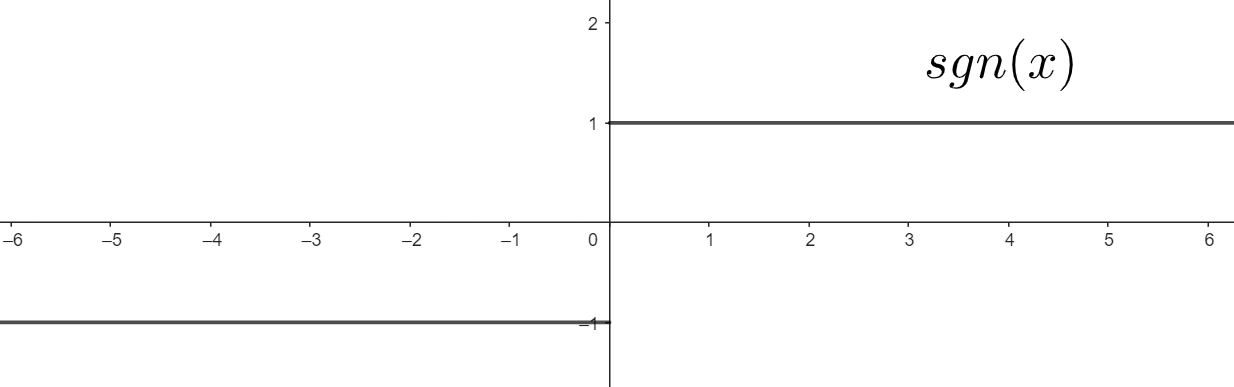
\includegraphics[scale=0.6]{Cours/sgn.png}
%     \caption{Fonction signe, dérivée de la valeur absolue. A noter qu'elle n'est pas définie en 0.}
%     \label{fig:enter-label}
% \end{figure}

\begin{proposition}\label{prop3}
La valeur absolue suit les propriétés suivantes: 
    \begin{enumerate}
  \item $x\leq |x|$;
  \item $|x|=0 \iff x=0$;
  \item $|xy|=|x||y|$;
  \item $|x+y|\leq |x|+|y|$ \, (inégalité triangulaire)
  % \item $|x-y|\geq ||x|-|y||$;
  % \item $|x|=x{\, \rm sgn}(x)$ \,\, $\forall \, x \neq0$
\end{enumerate}
\end{proposition}
\begin{proof}
    \textbf{ inégalité triangulaire: }
\\Cas d'égalité:
Si $a$ et $b$ sont de même signe, alors on a $|a+b|=|a|+|b|$.
\\Cas d'inégalité stricte: 
\\$|a+b|^2 = (a+b)^2 = a^2+b^2+2ab = |a|^2+|b|^2+2ab $
Or on sait que $ab\leq|ab|=|a||b|$, ce qui implique que
\\$|a+b|^2\leq|a|^2+|b|^2+2|a||b|=(|a|+|b|)^2$
\\et par croissance de la fonction carre, on obtient l'inégalité triangulaire. 
\end{proof}



\begin{tcolorbox}
    En mathématiques, la notion de mesure se réfère à la manière de quantifier la taille, la longueur, la superficie, le volume ou d'autres propriétés d'un ensemble de points ou d'objets dans l'espace. La mesure vise à attribuer des valeurs numériques à ces propriétés, ce qui permet de comparer et de caractériser les objets de manière précise. La théorie de la mesure est une branche des mathématiques qui étudie les concepts fondamentaux liés à la mesure, tels que la notion de "mesurable", les méthodes de construction de mesures et les propriétés des ensembles mesurables. Ce sujet sera plus amplement discuté en Algèbre mais nous voyons ici l'application de la mesure avec la valeur absolue.

    On peut alors utiliser la notion d'\textbf{espace métrique} qui sur $\Rr$ associe la distance usuelle. Ici notée $d$ était déjà utilisée par Euclide.
    \begin{defi} Distance usuelle:
        $\forall (x,y)\in\Rr ^2, d(x,y)=|x-y|$
    \end{defi}
    Cette distance est cruciale en analyse réelle et permet d'évaluer plusieurs propriétées importantes telles que la convergence ou la continuité. Pour ce faire, nous utiliserons la comparaison entre une distance et un nombre arbitrairement petit que l'on notera $\varepsilon$.
\end{tcolorbox}


\textbf{La notion d'epsilon}: 
Souvent en Analyse on utilise des grandeurs très petites pour définir des propriétés de limites, convergences et d'approximations. On choisit alors un une lettre $\varepsilon$ nommé "epsilon" pour représenter un nombre que l'on peut choisir et qui est aussi petit que l'on veut. Souvent les définitions commencent par: "$\forall \varepsilon>0$". On conclut alors intuitivement avec "peu importe à quel point la condition doit être satisfaite, on peut toujours trouver un epsilon suffisamment petit pour que la propriété soit vérifiée dans un voisinage des valeurs données". Ainsi en utilisant $\varepsilon$ on peut égaliser deux valeurs par des inégalités. 

\begin{proposition}
    Par exemple on peut montrer:
\begin{equation}
    a=b \iff |a-b|<\varepsilon \qquad \forall \varepsilon>0 {\,\, \rm et\,\, }\forall a,b \in \Rr
\end{equation}
\end{proposition}
\begin{proof}
    Nous devons prouver la double implication. \\D'abord de gauche à droite: Si $a=b$, alors pour tout $\varepsilon>0$, $|a-b|=0<\varepsilon$.
\\ \\Puis nous devons prouver de droite à gauche. Nous allons résonner par l'absurde. Supposons que $\forall \varepsilon>0$, $|a-b|<\varepsilon$. Supposons cette fois par l'absurde que $a\neq b$, c'est à dire $a-b\neq0$. Dans ce cas, nous pouvons choisir $\varepsilon = |a-b|/2$. Comme $a-b\neq 0$, $\varepsilon$ est strictement positif. Cependant, cela contredirait l'hypothèse selon laquelle pour tout $\varepsilon >0$, $|a-b|<\varepsilon$, car dans ce cas, $|a-b|$ ne pourrait être strictement inférieur à $|a-b|/2$. Donc, notre hypothèse initiale était fausse, et nous pouvons conclure que $a=b$.
\\ \\Ainsi, nous avons prouvé les deux implications ce qui montre l'équivalence.

\end{proof}




\subsection{Suites}
\begin{defi}
On appelle \textbf{suite numérique} (ou plus simplement \textbf{suite}) toute fonction de $\Nn$ dans $\Rr$, et on note 
\begin{equation}
    f: \Nn\longrightarrow\Rr,\; f(n):=x_n, \quad \forall n\in \Nn
\end{equation}
\end{defi}

Cette fonction associe a chaque entier naturel $n\in\Nn$ un élément de $\Rr$. La suite est donc l'ensemble de ce termes ($Im(f):=(x_n)_{n\in\Nn}\subset \Rr$), et on appelle $x_n$ le \textit{n-ième terme}, ou \textit{terme général} de la suite. Il est important de savoir que l'infini n'appartient pas aux réels, donc une suite peut tendre vers l'infini (voir plus tard la partie \ref{limite infinie suite}), mais aucun terme ne peut valoir l'infini.\\

On peut définir les suites de manière explicite: 
$x_n=f(n), \forall n\in\Nn$, ou par récurrence:
$ x_{n+1}=g(x_n), \; \forall n \in \Nn \text{ et } x_0 \in \Rr$.
De plus, on distingue deux types de suites particuliers:
\\Les suites arithmétiques se définissent explicitement par $x_n=x_0+n\cdot r, ~r\in\Rr$, et par récurrence: $x_{n+1}=x_n+r$.
\\Les suites géométriques se définissent explicitement par 
$x_n=x_0+r^n, r\in\Rr$ et par récurrence: $x_{n+1}=x_n\cdot r$.



Encore une petite définition concernant la monotonie des suites !


\begin{defi}
    On dit qu'une suite est :
    \begin{enumerate}
        \item constante si $\exists c\in \Rr $ tel que $x_n=c, \; \forall n \in \Nn $
        \item croissante si
        \[\forall n,m \in \Nn, ~~n\leq m\quad\implies\quad x_n\leq x_m \;  \]
        \item strictement croissante si
        \[\forall n,m \in \Nn, ~~n< m\quad\implies\quad x_n< x_m \]
        \item décroissante si
        \[\forall n,m \in \Nn, ~~n\leq m\quad\implies\quad x_n\geq x_m\]
        \item strictement décroissante si
        \[\forall n,m \in \Nn, ~~n< m\quad\implies\quad x_n> x_m \]
        \item monotone si elle est croissante ou décroissante
        \item strictement monotone si elle est strictement croissante ou strictement décroissante
    \end{enumerate}
\end{defi}

\subsection{Limites}
\begin{defi}
Soit $(x_n)_{n\in\Nn}\subset \Rr$. On dit que $l\in \Rr$ est la \textit{limite} de la suite  $(x_n)_{n\in\Nn}$ si 
\begin{equation}\label{definition limite}
    \forall \varepsilon>0, \; \exists N\in\Nn \; \text{ tel que } \; n\geq N \quad \implies \quad |x_n-l|<\varepsilon.
\end{equation}
On écrit alors 
\begin{equation*}
    \lim_{n\to\infty} x_n= l \text{ \quad ou \quad } x_n\longrightarrow l \; (n \rightarrow \infty),
\end{equation*}
et on dit que la suite \textit{converge} vers la limite $l$.     
\end{defi}
Décortiquons cette équation (\ref{definition limite}) ensemble pour y voir plus clair: 

"$\forall \varepsilon>0$": epsilon représente la distance entre les termes de la suites et la limite, donc la condition est vraie pour tout epsilon.

"$\exists N\in\Nn \; \text{ tel que } \; n\geq N$": il existe un entier naturel a partir duquel tous les termes de rang $n\geq N$ satisfont l'implication.

"$|x_n-l|<\varepsilon$": la distance entre le terme de rang $n$ et la limite est inférieure a tout epsilon arbitrairement petit.

En d'autres termes, il est astucieux de voir cette définition comme le fait qu'a partir d'un certain rang, on peut poser une limite $l\in\Rr$ telle que la distance entre les termes de la suite et la limite est très petite (d'où le concept d'epsilon).
Donc si on voit cela graphiquement: dans l'intervalle définit par $(l-\varepsilon,l+\varepsilon)$ tous les termes de la suite (sauf un nombre fini de 0 a \textit{N}) sont contenus dans l'intervalle, quelque soit epsilon.
Vous pouvez donc imaginer que dans ce cas, \textit{N} dépend de epsilon, d'où la notation \textit{N(}$\varepsilon$).
\\\textbf{Attention: } La limite $l$ est un nombre réel, i.e. $l\neq\pm\infty$. 


\begin{defi}
    Soit $(x_n)_{n\in\Nn}\subset \Rr$ une suite. On dit que $x_n$ est:
    \begin{enumerate}
        \item bornée inférieurement s'il existe $m\in \Rr$ tel que $x_n\geq m,\; \forall n\in\Nn$
        \item bornée supérieurement s'il existe $M\in\Rr$ tel que $x_n\leq M,\; \forall n \in\Nn$. On dit aussi que M est une borne supérieure de $x_n$.
        \item bornée si elle est bornée inférieurement et supérieurement
    \end{enumerate}
\end{defi}
\begin{proposition}Soit $(x_n)_{n\in\Nn}$ $\subset \Rr$:
\begin{enumerate}
  \item Si $x_n\longrightarrow l\in \Rr \quad(n\rightarrow\infty)$, alors la limite $l$ est unique
  \item Si $(x_n)_{n\in\Nn}$ converge, alors elle est bornée.
  \item S'il existe $n_0\in\Nn$ tel que $x_n=y_n$ pour tout $n\geq n_0$, alors les suites sont soit toutes deux convergentes soit toutes deux divergentes.
  \item Si $(x_n)_{n\in\Nn}$ et $(y_n)_{n\in\Nn}$ convergent et s'il existe $n_1\in \Nn$ tel que $x_n\leq y_n$ pour tout $n\geq n_1$, alors \[\lim_{n\rightarrow\infty}x_n\leq\lim_{n\rightarrow\infty}y_n\]
\end{enumerate}
\end{proposition}
\textbf{Preuve:}
(1) On raisonne par l'absurde:
On suppose qu'il existe deux limites $l$ et $l'$ distinctes telles que la suite $(x_n)_{n\in\Nn}$ vérifie: 
\\$\forall \varepsilon>0 ,\quad \exists N(\varepsilon)\in\Nn$ tel que $ \forall n \geq N(\varepsilon) \implies |x_n-l|<\frac{\varepsilon}{2}$
\\$\forall \varepsilon>0 ,\quad \exists N'(\varepsilon)\in\Nn$ tel que $ \forall n \geq N(\varepsilon) \implies |x_n-l'|<\frac{\varepsilon}{2}$
\\Donc, il est juste de supposer que d'à partir d'un certain rang, les deux conditions sont validées: pour tout $n\geq$ max{$N(\varepsilon), N'(\varepsilon)$}, on a
\begin{equation*}
    |l-l'|=|l-x_n+x_n-l'|\leq |x_n-l|+|x_n-l'|<\frac{\varepsilon}{2}+\frac{\varepsilon}{2}=\varepsilon
\end{equation*}
pour tout $\varepsilon>0$.
Donc $l=l'$.$ \square$
\hline
\hline
\newpage

\subsection{Principe des deux gendarmes}
\begin{theorem}
    Soit $(x_n)_{n\in\Nn}$, $(y_n)_{n\in\Nn}$, $(z_n)_{n\in\Nn}$ $\subset \Rr$. Supposons que:
\begin{enumerate}
    \item $\exists N \in \Nn$ tel que $x_n\leq y_n\leq z_n, \; \forall n\geq N$,
    \item $\lim_{n\rightarrow\infty}x_n=\lim_{n\rightarrow\infty}z_n=l$.
\end{enumerate}
Alors $\lim_{n\rightarrow\infty}y_n=l$.

\end{theorem}

\textbf{Preuve}: exercice.\\

% \begin{proof}
%     Soit $\varepsilon>0$.
% \\Puisque $\lim_{n\rightarrow\infty}x_n=\lim_{n\rightarrow\infty}z_n=l$, on peut trouver $n_0\in\Nn$, $n_0\geq n_0$, tel que:
% \begin{equation*}
%     x_n-l>-\varepsilon \quad et \quad z_n-l<\varepsilon, \forall n \geq n_0.
% \end{equation*}
% Alors on a 
% \begin{equation*}
%     -\varepsilon<x_n-l\leq y_n-l \leq z_n-l < \varepsilon, \forall n \geq n_0,
% \end{equation*}
% et ainsi $\lim_{n\rightarrow\infty}y_n=l.  $
% \end{proof}


Autrement dit, si une suite $(y_n)_{n\in\Nn}$ est bornée par deux suites $(x_n)_{n\in\Nn}$ et $(z_n)_{n\in\Nn}$ qui toutes les deux convergent vers la même limite, alors forcement la suite $(y_n)_{n\in\Nn}$ converge vers cette même limite comme tous ces termes sont compris entre les deux suites.\\

\textbf{Exemple:} on pose $(y_n)_{n\geq1}$ définie par $y_n=(1/n)sin(n^2)$, $\forall n \geq1$. 
\\On a:
\begin{equation*}
    -1\leq sin(n^2)\leq1 \implies \frac{-1}{n} \leq \frac{sin(n^2)}{n}\leq \frac{1}{n} , \quad \forall n \geq1
\end{equation*}
On remarque que $\lim_{n\rightarrow\infty}x_n=\lim_{n\rightarrow\infty}z_n=0$.
Donc par le théorème des gendarmes, la limite de $(y_n)_{n\geq1}$ est 0. \\

Pour illustrer cette situation et le théorème des gendarmes, voici un schéma qui montre les trois suites et leurs convergences:

\begin{figure}[H]
    \centering
    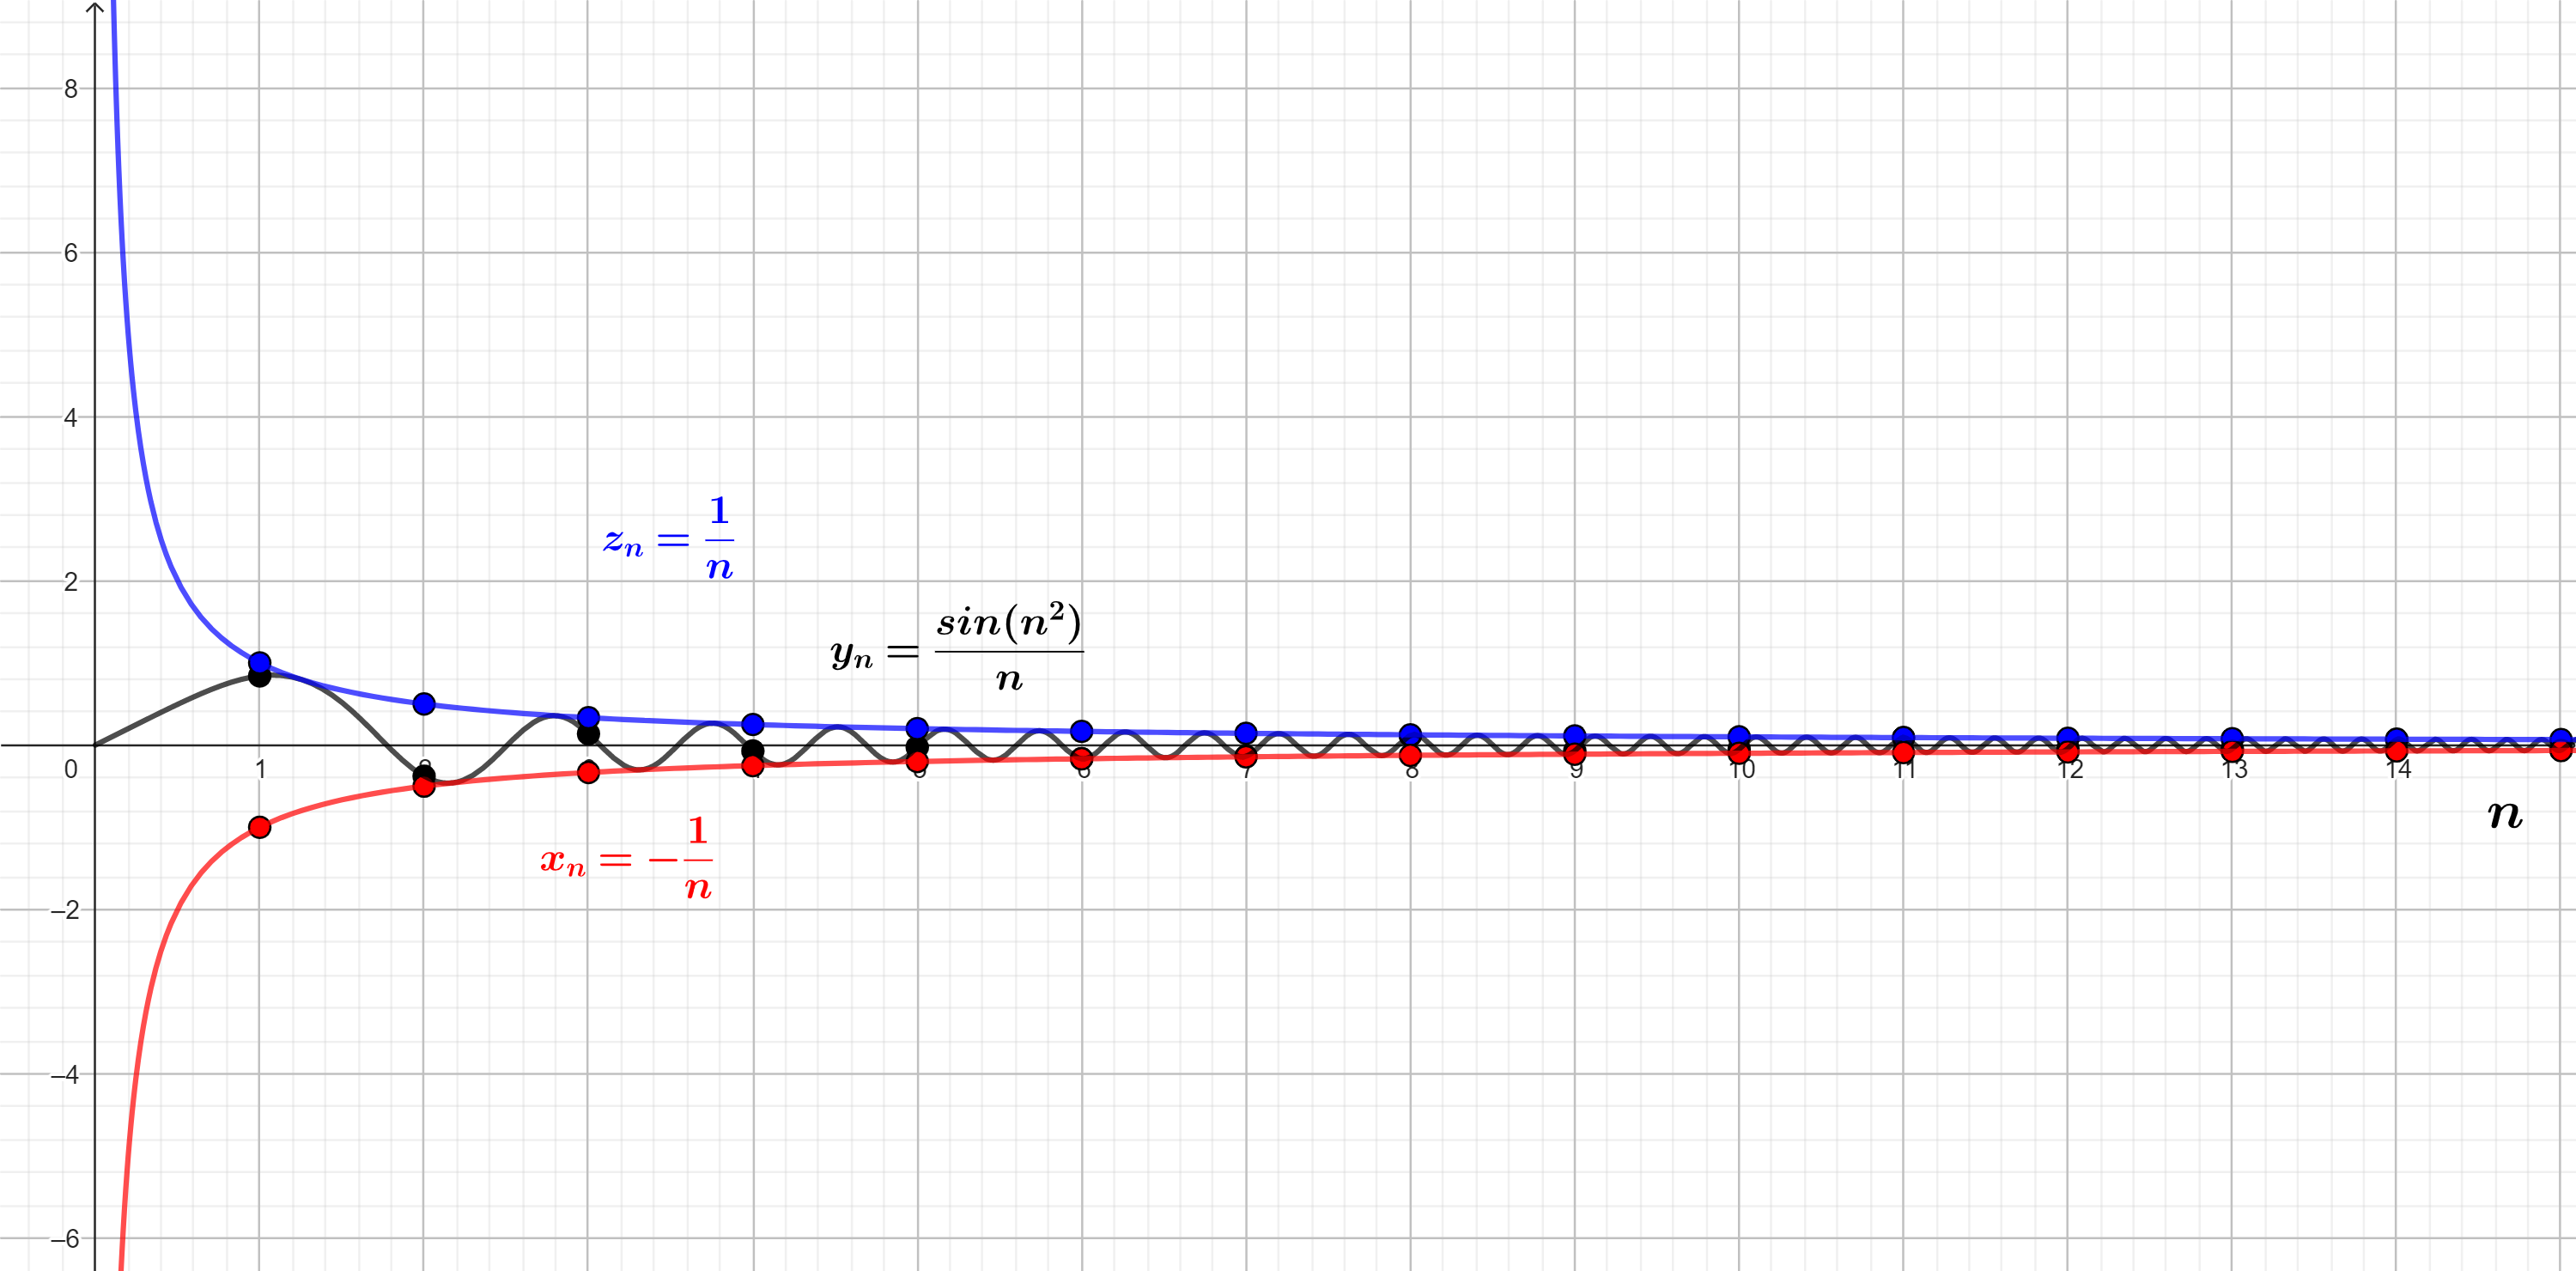
\includegraphics[scale=0.65]{Cours/gendarmes.png}
    \caption{La suite $y_n$ est bornée par deux suites qui convergent les deux vers 0. On voit que $y_n$ tend vers 0 aussi.}
    \label{fig:enter-label}
\end{figure}

% \begin{theorem}\label{4.5}
%     Soit $(x_n)_{n\in\Nn}$ $\subset \Rr$. Si $(z_n)_{n\in\Nn}$ est croissante (resp.décroissante) et bornée supérieurement (resp. bornée inférieurement), alors $(x_n)_{n\in\Nn}$ est convergente.
% \end{theorem}

% \paragraph{Preuve: exercice}

\newpage
\subsection{Extension du concept de limite: limite infinie}\label{limite infinie suite}
\begin{defi}
    

Soit $(x_n)_{n\in\Nn}$ $\subset \Rr$. On dit que 
\begin{equation*}
    \lim_{n\rightarrow\infty}x_n=+\infty
\end{equation*}
si
\begin{equation*}
    \forall M>0, \; \exists N=N(M)\in\Nn \quad\text{tel que} \quad x_n\geq M, \; \forall n\geq N,
\end{equation*}
On dit de même que 
\begin{equation*}
    \lim_{n\rightarrow\infty}x_n=-\infty
\end{equation*}
si
\begin{equation*}
    \forall M>0, \; \exists N=N(M)\in\Nn \quad \text{tel que} \quad x_n\leq -M, \;\forall n\geq N.
\end{equation*}
\end{defi}
\paragraph{Exemples}
\begin{enumerate}
    \item \[x_n=2^n, \quad \lim_{n\rightarrow\infty}x_n=\infty\]
    \item \[y_n=(-1)^n/n \quad \lim_{n\rightarrow\infty}y_n=0\]
    \item \[z_n=n*sin(n) \quad \lim_{n\rightarrow\infty}z_n \text{ n'existe pas.}\]  Cette suite est chaotique
    
\end{enumerate}
\begin{theorem}
    Soit $(x_n)_{n\in\Nn}$, $(y_n)_{n\in\Nn}$,  $\subset \Rr$.
\begin{enumerate}
    \item S'il existe $\delta >0$ et $n_0\in\Nn$ tel que $x_n\geq \delta$ pour tout $n\geq n_0$, et si $y_n\longrightarrow\pm \infty$, alors $x_ny_n\longrightarrow\pm\infty$ lorsque $n\longrightarrow\infty$
    \item Si $x_n\longrightarrow a\neq 0$ et $y_n\longrightarrow \pm \infty$, alors $x_ny_n\longrightarrow\pm$sgn$(a)\infty$ et $x_n/y_n\longleftrightarrow 0$ lorsque $n\rightarrow\infty$.
    \item Si $a>1$ et $x_n\Longrightarrow + \infty$, alors $a^{x_n}\rightarrow +\infty $ lorsque $n\rightarrow\infty$. 
\end{enumerate}
\end{theorem}
Ce que ce théorème explicite est que les valeurs compliquées en terme de limite sont 0 et les deux infinis. Si une suite tend vers une constante non nulle, alors l'autre suite va prendre l'ascendant lorsqu'elles sont multipliées. Par contre si on a une suite qui tend vers 0, l'autre vers l'infini, alors on ne peut conclue de façon général quant à la limite du produit. Donc attention aux raccourcis du type "$0\cdot \infty=0/\infty$"!\\


Tous ces théorèmes empilés les uns sur les autres sont peut être compliqués à comprendre rapidement ou alors ne paraissent être que des concepts faciles ou sans trop de sens, mais c'est ici qu'il faut savoir prendre le temps nécessaire pour se rendre compte du résultat et peut être faire le lien avec plus haut. Dans l'histoire des mathématiques aucun théorème ou proposition n'a été dicté sans être prouvée. C'est le propre des mathématiques. Prouver tous les théorèmes déjà existants en seulement 3 ans de bachelor est illusoire mais il s'agit d'en apprendre les plus intéressants ou les plus utiles pour notre futur dans les mathématiques théoriques ou appliquées. \\


\subsection{Les sous-suites}
Afin d'introduire la notion de \textit{sous-suite}, on peut commencer par s'intéresser au cas spécifique de la suite $a_n = (-1)^n$. Quelles informations pouvons-nous obtenir sur cette suite avec les outils obtenus jusqu'à maintenant ? 
Clairement cette série diverge. C'est un exercice intéressant de le montrer en utilisant correctement la définition $\varepsilon$ (Exercice facile ?). On peut par contre remarquer que la \textit{sous-suite} $a_{2n} = (-1)^{2n}$ est la suite constante égale à 1 qui est donc convergente. Naturellement, de la même manière la \textit{sous-suite} $a_{2n+1} = (-1)^{2n+1}$ est la suite constante égale à -1 et donc converge également. Le but de cette partie est d'alors de caractériser les suites, pas forcément convergente, pour lesquelles il existe des sous suites qui convergent. Nous commençons alors par définir proprement ce qu'est une \textit{sous-suite}.
\begin{figure}[H]
    \centering
    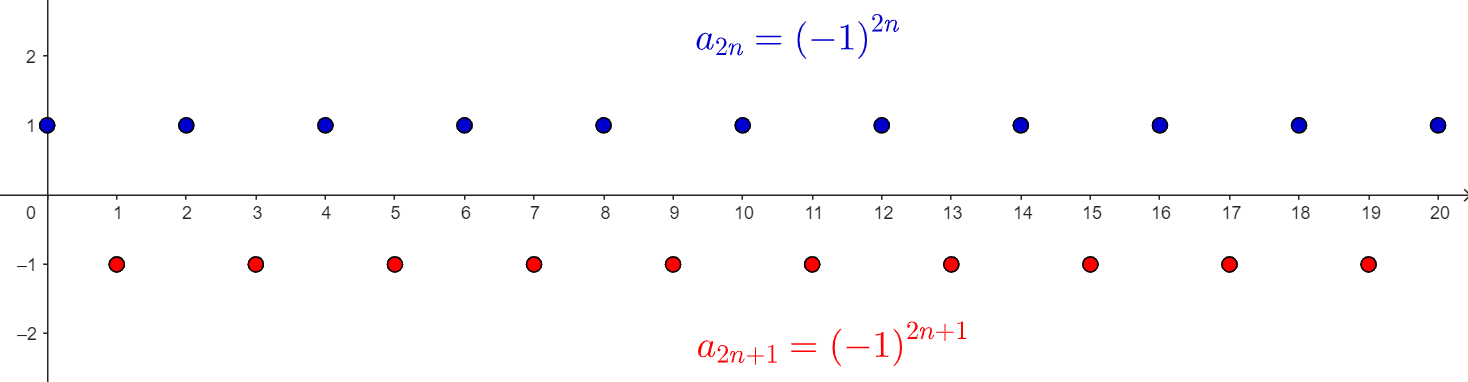
\includegraphics[scale=0.65]{Cours/a_n sous suite.png}
    \caption{Illustration de la suite $a_n = (-1)^n$ ainsi que les sous-suites $(a_{2n})$ et $(a_{2n+1})$ }
    \label{fig:enter-label}
\end{figure}

\begin{defi}
 Soit une suite $(x_n)_{ n \in \Nn } \subset \Rr $. On considère une fonction $\varphi : \Nn \rightarrow \Nn $ strictement croissante. On note alors $n_k := \varphi(k)$. Ainsi la suite $(x_{n_k})_{k \in \Nn} $ est appelée \textit{sous-suite} de  $(x_n)$. 
 \end{defi}
 
\textbf{Remarque :} La croissance stricte de la fonction $\varphi$ assure que l'ordre des termes de la sous suites est le même que dans la suite originale. De plus, il ne peut pas avoir de répétition des termes. 


\begin{proposition}\label{2}
    Toute sous-suite d'une suite convergente converge vers la même valeur que la suite d'origine.  
\end{proposition}
\textit{\textbf{Preuve}} Exercice 
\newline 
Bien que ce résultat peut paraître évident, il peut s'avérer utile dans la pratique afin de déterminer la valeur d'une limite. On donne ici un exemple simple qui pourrait s'appliquer à des exemple plus complexes.\later{ (à trouver pour un exo maybe )}\newline \\
\textbf{Exemple} Soit $0<b<1$, on considère la suite $(b_n) = b^n$. Clairement on peut voir que la suite et décroissante et bornée inférieurement. Ainsi le Théorème \ref{4.5}, assure que la suite $(b_n)$ est convergente. Alors, il existe  $l \in \Rr$ tel que $b > l \ge 0$ et $\lim_{n \to \infty} b_n = l$. Maintenant considérons la sous-suite $(b_{2n})$. D'un coté la proposition \ref{2} assure que $\lim_{n \to \infty} b_{2n} = l$, de l'autre on a que $b^{2n} = b_n^2$. Comme on a montré l'existence de la limite alors on conclut que $l = l^2$. L'unicité de la limite donne alors $l=0$. \\


\begin{defi}\label{def422}
On dit que $\lambda \in \Rr $ est un point d'accumulation d'une suite $(x_n)_{n \in \Nn} \subset \Rr$ si il existe une sous-suite qui converge vers $\lambda$.
\end{defi}
En reprenant à nouveau l'exemple de la suite $(x_n)_{n \in \Nn} = (-1)^n$ on peut alors conclure à partir de la définition précédente que -1 et 1 sont des points d'accumulations de la suite non-convergente $(x_n)$.  
 
\begin{theorem}{\textbf{Bolzano-Weierstrass 1874}}
    Toute suite bornée admet au moins une sous-suite convergente. 
\end{theorem}
La preuve qui ne sera pas détaillée ici utilise le lemme suivant qui peut s'avérer utile:

\begin{lemma}
\label{peak point lemma}
    Toute suite admet une sous-suite monotone.
\end{lemma}


% \textit{\textbf{Preuve:}} Soit une suite $(x_n)_{n\in \Nn}.$ On peut alors distinguer deux cas. 

% Le premier si l'on suppose que pour tout $N > 0,$ l'ensemble $\{x_n : n > 
% N\}$ a un maximum. Alors on peut définir une sous suite de la manière 
% suivante:
% \begin{itemize}
%     \item $x_{n_1} = max\{x_n : n > 1\}$
%     \item $x_{n_2} = max\{x_n : n > n_1\}$
%     \item $x_{n_3} = max\{x_n : n > n_2\}$
    
% \end{itemize}
% Et ainsi de suite. On remarque que $n_1$ correspond à l'indice du maximum de l'ensemble des valeurs de la suite, et on choisi le première valeur de notre sous-suite la valeur associer à l'indice $n_1.$ 
% Pour la prochaine valeur de notre sous-suite on doit prendre une valeur qui a un indice $n_2,$ tel que $n_1 < n_2.$ 
% Et alors pour la deuxième valeur de notre sous-suite nous prenons le maximum des valeurs de la suite dont l'indice correspondant est strictement plus grand que $n_1.$ 
% Et on continue ainsi de suite pour construire une sous-suite qui est décroissante. 

% Maintenant on s'intéresse au cas où il n'est pas vrai que pour tout $N>0$ l'ensemble $\{x_n : n > N\}$ a un maximum.
% Alors il existe $N_1 > 0$ tel que l'ensemble $\{x_n : n > N_1\},$ n'a pas de maximum. 
% Alors pour tout élément de la suite $x_m,$ tel que $m > N_1$ on peut trouver un élément de la suite $x_n > x_m,$ tel que $n > m.$
% Car s'il n'existe aucun élément $x_n > x_m,$ avec $n > m,$ ça veut dire que l'on peut définir un maximum pour l'ensemble $\{x_n : n > N_1\},$ qui serait $max\{x_{N_1 +1}, \ldots, x_m\}.$ 
% Mais cela contredit l'hypothèse que $\{x_n : n > N_1\},$ n'a pas de maximum.
% Alors on définit une sous suite tel que $x_{n_1} = x_{N_1 + 1}.$ \\
% $x_{n_2}$ est le premier élément qui suit $x_{n_1},$ tel que $x_{n_1} < x_{n_2}.$\\
% $x_{n_3}$ est le premier élément qui suit $x_{n_2},$ tel que $x_{n_2} < x_{n_3}.$\\
% Et ainsi de suite. On a alors définit une sous-suite décroissant. 

% Alors on peut soit extraire une sous-suite croissante ou décroissante et donc qu'il existe une sous-suite monotone. $\Box$\\
 
% Alors maintenant on prouvera le Théorème Bolzano-Weierstrass. \\
% \textit{Preuve:} On peut extraire une sous-suite monotone par le lemme \ref{peak point lemma} 
% La suite étant borné implique que notre sous-suite monotone est aussi borné. Alors par le Théorème \ref{4.5} la sous-suite converge.$\Box$

Ce théorème semble très abstrait ici. Mais vous pouvez l'imaginer par le fait que si nous avons un nuage de points qui est compris entre deux bornes, on peut trouver un suite dans ces points qui convergent vers une valeur. Pensez simplement à une sous-suite constante qui peut exister dans les suites périodiques, soit les suites qui se répètent avec la même fréquence.

Ce théorème est néanmoins très utilisé lors de démonstrations avec les suites afin de trouver une suite qui converge. Pour preuve, il sera utilisé plus bas avec les suites de Cauchy!

\subsection{Suites de Cauchy et espace complet}
\begin{defi}{\textbf{Suites de Cauchy}} 
   On dit qu'une suite $(x_n)_{n \in \Nn} \subset \Rr $ est de Cauchy si $\forall \varepsilon >0 $, $\exists \: N(\varepsilon) \in \Nn $ tel que $\forall \: m,n \ge N(\varepsilon)$ on a que $|x_n - x_m| < \varepsilon$.  
\end{defi}
Intuitivement on dira qu'une suite est de Cauchy si les termes de la "queue" de la suite sont arbitrairement proche entre eux (i.e $\varepsilon$-proche).  On parle de la "queue" de la suite pour désigner les termes qui on un indice $n$ très grand. La queue possède un nombre infini d'éléments de la suite.  Si tous les termes finissent par être très proche entre eux on peut imaginer que la suite converge. On énonce maintenant un critère de convergence d'une suite. 


\begin{theorem}\label{thm420}
Une suite réele est convergente si et seulement si elle est de Cauchy.
\end{theorem}

\textit{\textbf{Preuve:}} \newline 
"$\implies$"
     Soit une suite $(x_n)_{n\in \Nn},$ qui converge vers $L\in \Rr.$ C'est à dire 
    \[
    \forall \varepsilon>0, \; \exists N(\varepsilon) >0 \; \text{ tel que } \; \forall n\geq N \quad |x_n-L|<\varepsilon.
    \]
    Alors soit $N'>0,$ tel que pour tout $n > N',$ on a que   $ |x_n - L| < \frac{\varepsilon}{2}$

    Alors en écrivant 0 de manière convenable on a que $\forall n,m \ge N(\varepsilon)$ :
    $$ |x_n - x_m| = | x_n -L + L -x_m| \le |x_n - L | + | x_m -L | < \frac{\varepsilon}{2} + \frac{\varepsilon}{2} = \varepsilon,$$
    où on a utilisé l'inégalité triangulaire. \newline 
" $\impliedby$" Là où l'implication à droite était relativement facile à montrer, le chemin pour démontrer la réciproque est un peu plus subtile. On va monter que toute suite de Cauchy est bornée et ensuite par Bolzano-Weierstrass, nous montrerons que la limite de la suite correspondra à la limite de la sous-suite convergente extraite par BW en utilisant à nouveau un "jeu" avec des $\varepsilon$. Commençons par énoncer et prouver le lemme suivant. 
\begin{lemma}\label{lem46}
    Si une suite est de Cauchy alors elle est bornée. 
\end{lemma}  
\textit{\textbf{Preuve}} Par hypothèse la suite est de Cauchy. Soit $\varepsilon >0 $ arbitraire, on a alors qu'il existe un certain rang $N(\varepsilon)$ tel que $\forall m,n \ge N(\varepsilon)$ on a $|x_n-x_m| < \varepsilon$. En particulier, en prenant $m = N(\varepsilon)$, on obtiendra les inégalités suivante $x_N - \varepsilon < x_n < x_N + \varepsilon$. Il suffit alors de poser les bornes suivantes : 
$$ a := min \{x_0, x_1, ..., x_N, x_N - \varepsilon \} \;\;\; b := max \{x_0, x_1, ..., x_N, x_N + \varepsilon \}. $$
pour obtenir directement des inégalités indépendantes du choix du $\varepsilon$, $a \le x_n \le b $ $ \forall n \in \Nn$. $\Box$ \\ \newline
On peut à présent retourner à la preuve du \ref{thm45}. Le lemme \ref{lem46} nous permet d'invoquer le fameux théorème de Bolzano-Weierstrass (BW) dont nous avons discuté auparavant. 
Le théorème affirme ainsi l'existence d'une sous-suite $\{x_{n_k}\}_{k\in\Nn},$ qui converge vers un certain $L\in \Rr.$ Alors on veut montrer que notre suite $(x_n)$ converge bien vers $L.$
À nouveau soit $\varepsilon > 0,$. Par la convergence de la sous-suite nous un rang $N > 0,$ tel que pour tout $k > N,$ on a que $|x_{n_k} - L| < \varepsilon.$ Alors maintenant considérons la convergence. Soit $n > n_k,$ avec $k > N$ alors on a:
\[
|x_n - L| < |x_n - x_{n_k}| + |x_{n_k} - L| < 2\varepsilon,
\]

en ayant utilisé le fait que la suite soit de Cauchy et la convergence de la sous-suite. Ce qui conclut la preuve. $\Box$   
\newline 
\newline 

\textit{\textbf{Pour aller plus loin...}}
Le théorème affirme que l'espace normée $(\Rr, |.|)$ est un espace complet. La notation $(\Rr, |.|)$ dénote que l'on considère la structure de l'ensemble des réels muni de la métrique qui est la valeur absolue par la proposition (\ref{prop3}), une telle structure est appelée espace métrique. De manière intuitive on dit qu'un espace est complet s'il n'a pas de "trou". La condition plus formelle de la complétude d'un espace métrique est donc donnée par le théorème précèdent. 

\subsection{Limite Inférieur et Limite Supérieur d'une Suite}
On peut voir d'après le lemme \ref{lem46} qu'une suite qui converge est 
borné. Mais l'implication inverse n'est pas toujours vraie. On aimerait par contre pouvoir estimer par "combien" une suite borné diverge. 
Pour cela on peut s'intéresser à la notion de limite supérieur et limite inférieur d'une suite.

\begin{defi}
    Soit $\{x_n\}_{n\in \Nn}$ une suite borné. Alors posons  les suites $\{t_n\}_{n\in\Nn},$ et $\{s_n\}_{n\in \Nn}$ tel que:
    \[
    t_n = \sup\{x_k \; : \; k > n\}
    \]
    \[
    s_n = \inf\{x_k \; : \; k > n\}
    \]
    Ces deux suites, $\{t_n\}$ et $\{s_n\}$ converge toutes les deux 
    étant donné qu'elle sont monotone et borné. Et alors on définit la 
    limite supérieur de la suite $\{x_n\},$ comme la limite de la suite 
    $\{t_n\}, $ et la limite inférieur de la suite $\{x_n\},$ comme la 
    limite de la suite $\{s_n\}.$ On écrit alors 
    \[
    \limsup_{n \rightarrow \infty} x_n = \lim_{n \rightarrow \infty} t_n
    \]
    \[
    \liminf_{n \rightarrow \infty} x_n = \lim_{n \rightarrow \infty} s_n
    \]
    
\end{defi} 
Il est important de noter que $\{t_n\}$ et $\{s_n\}$ ne sont pas nécessairement des sous-suites de $\{x_n\}.$ 

\begin{figure}[H]
    \centering
    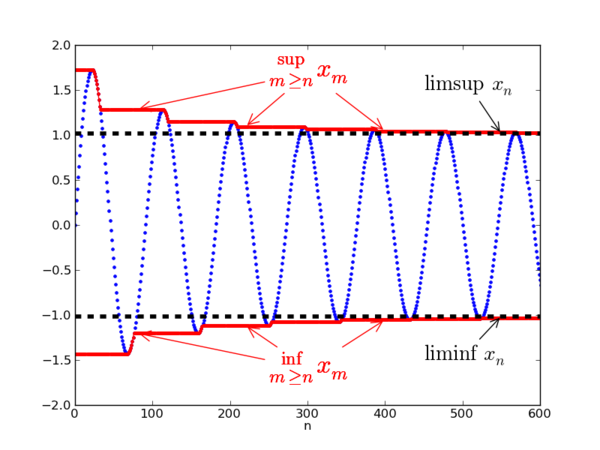
\includegraphics[scale=0.65]{Cours/Lim_sup_example_5}
    \caption{Une illustration du $\limsup$ et $\liminf.$ 
    On voit ici que la suite $x_n$ ne converge pas mais la suite des suprémums converge et la suite des infimums converge. Les deux sont en rouge et bornent la suite $x_n$.}
    \label{fig:enter-label}
\end{figure}

\textbf{Exemple} Soit la suite $\{x_n\}_{n\in \Nn},$ définie tel que $x_n = sin(n).$ Alors $limsup \; x_n = 1,$ et $liminf \; x_n = -1.$ (Ceci est vrai car la suite est équidistribuée avec une période de 2 $\pi$)

On peut également donner une définition alternative des limites inférieures et supérieures en considérant l'ensemble des points d'accumulation. 
\begin{defi}
    Soit une suite $\{x_n\}_{n\in \Nn}\subset \Rr$. On note $E$ l'ensemble de ses point d'accumulation, c'est à dire l'ensemble des $x_*$ tel qu'il existe une sous-suite $\{x_{n_k}\}$ qui converge vers $x_*$. Ainsi on définit,
        \[
    \limsup_{n \rightarrow \infty} x_n = \sup E
    \]
    \[
    \liminf_{n \rightarrow \infty} x_n = \inf E
    \]
\end{defi}
 Ainsi on remarque que ces nombres peuvent éventuellement être infini. 
En prenant la suite $x_n=\sin(\frac{n}{2}\pi)\cdot n, ~ n\in \Nn$, on voit que celle-ci diverge. En effet, le sinus oscille et cela donne plusieurs points d'accumulations.

Prenons la sous-suite $x_{2n}=0$. Elle est constante et converge donc vers 0 à l'infini

Considérons maintenant la sous-suite $x_{1+4n}=sin(\frac{1+4n}{2}\pi)(1+4n)=sin(\frac{\pi}{2}+2n\pi)(1+4n)=(1+4n)$. Celle-ci tend vers $\infty$. 

Finalement, considérons la sous-suite $x_{3+4n}=sin(\frac{3+4n}{2}\pi)(3+4n)=sin(\frac{3\pi}{2}+2n\pi)(3+4n)=-(3+4n)$. Celle-ci tend vers $-\infty$.

Nous venons de voir qu'il y a au moins 3 points d'accumulation qui sont 0, $\infty$ et $-\infty$. Notez le " au moins " car notre analyse ne permet pas de déduire si nous les avons tous trouvés! 


\section{Chap 3} \textbf{PRECISER ABSOLUMENT (meme juste à l'oral) LES EXEMPLES DE 1/n^2 et 1/n}
Dans ce chapitre nous allons étudier des nouveaux objets : les séries numériques. En se basant sur la théorie développée au chapitre précèdent sur les suites nous allons énoncer quelques critères de convergence pour ces sommes infinies. Nous commençons par énoncer les définitions formelles. 
\subsection{Définition et introduction}
\begin{defi}
    Soit une suite $(a_n)_{n \in \Nn } \subset \Rr$ une série numérique est une expression de la forme : 
    $$ \sum_{n=0}^{\infty} a_n = a_0 + a_1 + a_2 + a_3 + ... $$
 \end{defi}    
On parle ainsi aussi de sommes infinies. La question tout à fait naturelle à se poser en voyant cet objet est donc est ce que l'on peut écrire $\sum_{n=0}^{\infty} a_n = s \in \Rr $ ? On dira que la série converge vers $s \in \Rr$ si c'est le cas. On définira cette idée de convergence proprement dans la définition suivante.
\newline 
Comme nous avons à priori aucun outil pour étudier cet objet nous allons travailler de sorte à pouvoir utiliser les outils développés pour les suites. Nous définissons ainsi les \textit{suites de sommes partielles}. 
\begin{defi}
    Pour une série  $ \sum_{n=0}^{\infty} a_n$, on définit la suite des sommes partielles comme étant la suite $(s_m)$ définie par : $$ s_m = \sum_{n=0}^m  a_n = a_0 + a_1 + a_2 + a_3 + ... + a_m $$
    Pour clarifier la nature de l'objet explicitons les premiers termes de la suite :
    $$ s_0 = a_0$$
    $$ s_1 = a_0 + a_1$$
    $$ s_2 = a_0 + a_1 + a_2$$
    $$ s_3 = a_0 + a_1 + a_2 + a_3$$
    et ainsi de suite.
    On dit que la série  $ \sum_{n=0}^{\infty} a_n$ converge vers  $ s\in \Rr$ si la suite des sommes partielles converge vers $s \in \Rr$. On appelle alors $s$ la valeur de la série. Dans le cas où la suite de sommes partielles ne converge pas on dira que la série diverge. 
\end{defi}

Essayons ainsi d'étudier la convergence d'une série en utilisant les résultats du chapitre suivant sur la suites des sommes partielles. \newline
\textbf{Exemple :} Considérons la série $\sum_{n=1}^{\infty} \frac{1}{n^2}$. On notera alors la suite des sommes partielles correspondante comme : $$ s_m = \sum_{n=1}^{m} \frac{1}{n^2} = 1 +  \frac{1}{4} + \frac{1}{9} + .. + \frac{1}{m^2}.$$
Ainsi, on peut conclure que les termes de la suites sont strictement positifs. Ainsi on aura que $s_{m+1} - s_m = \frac{1}{(m+1)^2} > 0$. D'où la suite $s_m$ est croissante. En effet si une série est à termes positifs alors la suite des sommes partielles est forcément croissante. On souhaite pouvoir utiliser ainsi le résultat du théorème \ref{4.5} afin de montrer que la série converge. Nous cherchons alors à borner supérieurement la suite des sommes partielles. Comme souvent en analyse, pour trouver une borne sup/inf nous cherchons à réécrire les terme de notre expression d'une manière "convenable", ce genre de passages peuvent paraître parfois un peu "tiré par les cheveux" mais il faut toujours garder un esprit créatif lorsque l'on fait de l'analyse. Observons alors que $$ s_m = 1 + \frac{1}{2\cdot2} + \frac{1}{3\cdot3} + ... + \frac{1}{m \cdot m} < 1 + \frac{1}{2\cdot1 } + \frac{1}{3\cdot2} + ... + \frac{1}{m \cdot (m-1)}$$
$$= 1 + \left ( 1 - \frac{1}{2} \right ) + \left ( \frac{1}{2} - \frac{1}{3} \right ) + \left ( \frac{1}{3} - \frac{1}{4} \right ) + ... + \left ( \frac{1}{m-1} - \frac{1}{m} \right ) .$$
Remarquons alors que les termes de notre borne supérieure s'annulent de "proche en proche". C'est à dire qu'il reste que le premier et le dernier terme de la suite qui se n'annulent pas alors que les autres s'annulent entre eux. Il s'agit en fait d'une \textit{somme télescopique}. On a donc finalement que : 
$$ s_m < 1+1-\frac{1}{m} < 2. $$ Nous pouvons donc finalement conclure que la suite des sommes partielles est croissante et bornée par 2 supérieurement. Ainsi par le théorème \ref{4.5}, on conclut que la série converge vers une valeur inconnue plus petite que 2. Le calcul de cette série est plus connu sous le nom du problème de Bâle. Ce problème fut résolu par le mathématicien et physicien suisse, Leohnard Euler en 1735, il montra que : $\sum_{n=1}^{\infty} \frac{1}{n^2} = \frac{\pi^2}{6}$. 
\newline 
On peut résumer les quelques notions que nous avons observé précédemment dans la remarque suivante. \newline 
\textbf{Remarque:}  
 Pour une série à termes positifs alors la suite des sommes partielles est croissante. Ainsi soit la suite est bornée et ainsi la série converge vers son supremmum, ou bien la série diverge. \newline 
Essayons ainsi d'étudier la convergence de la série harmonique de la même manière. 
 \newline
\textbf{Exemple :} Considérons cette fois ci la série $\sum_{n=1}^{\infty} \frac{1}{n}$. On a de nouveau une série à termes positifs donc la suites des sommes partielles est croissante. On peut alors chercher à borner supérieurement cette suite. On remarque directement que 2 n'est plus une borne supérieure comme :
$$ s_4 = 1 + \frac{1}{2} + \frac{1}{3} + \frac{1}{4} > 1 + \frac{1}{2} + \frac{1}{4} + \frac{1}{4} = s_2 + \frac{1}{2} = 2. $$ 
Enfait on peut monter que la suite ne peut pas être bornée. En effet, en utilisant le même style d'astuce que dans l'exemple précèdent on a que :
$$ s_{2^k} = 1 + \frac{1}{2} + \left (\frac{1}{3}+ \frac{1}{4} \right ) + \left( \frac{1}{5} + ... + \frac{1}{8} \right ) + ... + \left( \frac{1}{2^{k-1}+1} + ... + \frac{1}{2^k} \right ) $$
$$ >  1 + \frac{1}{2} + \left (\frac{1}{4}+ \frac{1}{4} \right ) + \left( \frac{1}{8} + ... + \frac{1}{8} \right ) + ... + \left( \frac{1}{2^{k}} + ... + \frac{1}{2^k} \right ) $$
$$ =  1 + \frac{1}{2} + 2\left (\frac{1}{4} \right ) + 4\left( \frac{1}{8} \right ) + ... + 2^{k-1} \left( \frac{1}{2^{k}} \right ) = 1 + k \left (\frac{1}{2} \right ) = s_1 + k \left (\frac{1}{2} \right )$$
Ce qui donne donc que $s_{2^k} >  s_1 + k \left (\frac{1}{2} \right ) $. Ainsi par la croissance de la suite des sommes partielles on a alors que $\forall M > 0$, $\exists m_0$ tel que $\forall n > 2^{m_0}$ on a $s_n \ge s_{N_0} \ge M$. Donc on a que $s_m \rightarrow \infty$. Autrement dit la série harmonique est divergente. \newline 
Ces deux exemples pourtant similaires montrent que deux séries pourtant visiblement pas si différentes l'une de l'autre se comportent de manière totalement différente à l'infini. En fait, on remarque que les deux séries ont des termes qui tendent vers 0 à l'infini i.e $\frac{1}{n} \rightarrow \infty$ et $\frac{1}{n^2} \rightarrow \infty$ lorsque $n \rightarrow \infty$. En effet pour une série convergente $\sum_{n=0}^{\infty} a_n$ alors nécessairement $\lim_{\to \infty} a_n = 0$. Il s'agit d'une condition nécessaire à la convergence mais pas suffisante comme nous l'observons. Il faut alors que ces termes tendent "suffisamment vite" vers 0 afin que la série converge. 
\newline
\\Nous allons énoncer maintenant quelques proposition pour caractériser la convergence des séries et enfin énoncer des critères de convergence.
Commençons par donner une condition nécessaire et suffisante à la convergence d'une série.
\begin{proposition}
    Une série $\sum_{n = 0}^{\infty} a_n$ est convergente si est seulement si 
    \\\quad $ \forall \varepsilon > 0$, $\exists N(\varepsilon) \in \Nn $ tel que $\forall n > N(\varepsilon)$ et $\forall p \in \Nn $ alors $|a_n + ... + a_{n+p}| < \varepsilon$. 
\end{proposition}
\begin{proof}
   On sait qu'une série converge si et seulement la suite des sommes partielles converge donc par le théorème \ref{thm420} alors on a que la suite des sommes partielles doit être de Cauchy. D'où $\forall \varepsilon >0 $, $\exists N(\varepsilon)$ tel que $\forall p$ et $\forall n \ge N(\varepsilon)$ alors $|s_{n+p} - s_n| = | a_n + .. + a_{n+p}| < \varepsilon$ 
\end{proof}
Notons que dans ce style de démonstration, il faut être prudent à éviter la confusion entre les $a_n$ qui désignent les termes de la série et les $s_m$ qui désignent les termes de la suites des sommes partielles. 
\later{ajouter intro ou transition}
%\\De plus, il est important de noter que la convergence implique que la suite a une limite nulle, mais le contraire n'est pas forcement vrai
\begin{proposition}
    Si $\sum_{n=0}^{\infty} x_n$ est une série convergente, alors $\lim_{n\rightarrow\infty}x_n=0$.
\end{proposition}
 La réciproque est bien évidemment fausse comme nous l'avons vu avec la série harmonique. 
\begin{defi}
    On dit qu'une série $\sum_{n=0}^{\infty} x_n$ est absolument convergente si $\sum_{n=0}^{\infty} |x_n|$ est convergente.
\end{defi}

\begin{proposition}
    Si une série est absolument convergente, alors elle est convergente.
\end{proposition}
\newline 
\\ \textbf{Remarque :} Notons que la réciproque de cette proposition est bien évidemment fausse. \newline 
\hline 
\hline
\newpage
\subsection{Critères de convergence}
\later{comparaison, d'alembert, et cauchy (racine)}
\begin{theorem}
    (1er critère de comparaison)
    Soit $(x_n)_{n\in\Nn}$, $(p_n)_{n\in\Nn}\subset\Rr$ avec $p_n\geq0$ pour tout $n\in\Nn$.
    On a alors deux critères:
    \begin{enumerate}
        \item S'il existe $n_0 \in\Nn$ tel que $|x_n|\leq p_n$ pour tout $n\geq n_0$ et si la série $\sum_{n=0}^\infty p_n$ est convergente, alors la série $\sum_{n=0}^\infty x_n$ converge absolument.
       \item S'il existe $n_0 \in\Nn$ tel que $|x_n|\geq p_n$ pour tout $n\geq n_0$ et si la série $\sum_{n=0}^\infty p_n$ diverge, alors la série $\sum_{n=0}^\infty |x_n|$ diverge .
    \end{enumerate}
\end{theorem}

\begin{theorem}
    Soit $(x_n)_{n\in\Nn}$, $(p_n)_{n\in\Nn}\subset\Rr$ avec $p_n\geq0$, $x_n\neq 0$ pour tout $n\in\Nn$. 
    \begin{enumerate}
        \item S'il existe $n_0\in\Nn^*$ tel que
        \begin{equation*}
            |\frac{x_{n+1}}{x_n}|\leq \frac{p_{n+1}}{p_n}, \forall n \geq n_0-1
        \end{equation*}
        et si $\sum_{n=n_0}^\infty p_n$ est convergente, alors la serie $\sum_{n=0}^\infty x_n$ converge absolument.
    \end{enumerate}
\end{theorem}

\begin{theorem}
    Soit $(x_n)_{n\in\Nn}$, $(p_n)_{n\in\Nn}\subset\Rr$ avec $p_n\geq0$ pour tout $n\in\Nn$.
\end{theorem}
\section{Chap 4}
Comme expliqué plus haut, l'analyse est une branche des mathématiques qui étudie l'infinitésimal. On s'intéresse donc aux limites. Nous avons vu les limites au travers des suites et des séries. Nous allons maintenant nous intéresser aux fonctions afin d'étudier les limites au travers de la continuité. Ce chapitre sera rempli notamment de définitions car la continuité n'est bien évidemment pas seulement le fait de pouvoir "tracer la courbe sans lever le stylo". Ces notions sont d'une importance capitales et donc il est nécéssaire, comme toujours en maths, de bien poser les bases.

\subsection{Rappels}
Commençons par quelques rappels sur les fonctions: 
\begin{defi}
    Soit $D\subset \Rr$ un sous ensemble de $\Rr$. On définit une correspondance qui à un nombre $x\in D$ associe un unique $y\in \Rr$. On dit qu'une telle correspondance est une fonction définie sur $D$. On note $f$ cette fonction, $f(x)$ sa valeur $y$ en $x$ et $D=D(f)$ son domaine de définition: 
    \begin{align*}
        f\; : \; D(f)&\longrightarrow \Rr\\
        x\; &\longrightarrow f(x)=y
    \end{align*}
  On dit que $y$ est l'image de $x$ par la fonction $f$ et que $x$ est un antécédent de $y$. On notera Im$(f)$ l'ensemble suivant Im$(f)=\{y\in \Rr : \exists x \in D(f) \text{ tel que } f(x)=y\}$.On l'appelera image de $f$.

\end{defi}
\begin{rem}
 Petit rappel, la définition de l'image se lit comme suit "L'image de $f$ est défini par l'ensemble des $y$ réels tel qu'il existe un nombre $x$ dans l'ensemble de définition de la fonction $f$ tel que $f(x)=y$". La notation mathématique est très utile, vous le voyez....     
\end{rem}
 
\begin{defi}
    Nous définissons les opérations élémentaire sur les fonctions. Soient $f,g$ deux fonctions et $D(f), D(g)$ leur domaine de définitions respectifs. 
    \begin{enumerate}
        \item \textbf{Addition:} $(f+g)(x)=f(x)+g(x)$ ,$\forall x \in D(f)\cap D(g)$.
        \item \textbf{Multiplication par un scalaire:} $(\alpha f)(x)=\alpha f(x)$ $\forall x\in D(f)$ et $\alpha$ un scalaire.
        \item \textbf{Produit:} $(f\cdot g)(x)=f(x)\cdot g(x)$ ,$\forall x \in D(f)\cap D(g)$.
        \item \textbf{Quotient:} $\frac{f}{g}(x)=\frac{f(x)}{g(x)}$ ,$\forall x \in D(f)\cap D(g)$ et tel que $g(x)\neq 0$.
        \item \textbf{Composition:} $(f\circ g)(x)=f(g(x))$ ,$\forall x \in D(g)$ tel que $g(x)\in D(f)$.
    \end{enumerate}
    De plus, on notera $f\leq g$ si $f(x)\leq g(x)$ ,$\forall x \in D(f)\cap D(g)$. De même pour l'inégalité stricte. 
\end{defi}
Les définitions suivantes sont assez similaires à celles pour les suites. Néanmoins, une des majeures différences entre les suites et les fonctions est que le domaine de définition des suites est discret là où celui des fonctions peut-être continu. En effet, les suites prennent des nombres $n\in \Nn$ là où les fonctions peuvent prendre des valeurs dans tous les réels par exemple. Il va donc falloir que l'on crée des conditions sur ce $x$ car il peut être continu.

On va maintenant décrire le principe de voisinage qui vous servira plus tard.
\begin{defi}Soit $f\;:\; D(f)\longrightarrow \Rr$, une fonction: 
\begin{enumerate}
    \item On dit que $f$ est définie au voisinage de $a\in \Rr$ s'il existe $\delta >0$ tel que $(a-\delta,a+\delta)\subset D(f)\cup\{a\}$
    \item De façon générale, un voisinage de $a$ est un intervalle ouvert contenant le point $a$. On parle de $\delta $-voisinage pour un intervalle ouvert de la forme $(a-\delta,a+\delta)$. 
    \item On appelle voisinage pointé de $a$ un voisinage privé du point $a$, i.e. un sous-ensemble de $\Rr$ de la forme $I\setminus \{a\}$ où $I$ est un voisinage de $a$.
    \item On parle de voisinage à gauche de $a$ pour les sous-ensembles de $\Rr$ de la forme $(a-\delta,a],\; \delta>0$ et on définit naturellement le voisinage à droite de façon analogue ainsi que le voisinage pointé à gauche (resp. à droite).
    \item On dit que $f$ est définie au voisinage de $+\infty$ s'il existe $A>0$ tel que $(A,+\infty)\subset D(f)$, avec une définition "symétrique" au voisinage de $-\infty$.
\end{enumerate}
\end{defi}

Maintenant, dans l'ensemble des images d'une fonction on peut trouver quelques points spéciaux qui sont soit des maximaux soit des minimaux...
\begin{defi}
Soit $f$ une fonction et $D(f)$ son domaine de définition. 
\begin{enumerate}
    \item On dit que $f$ est bornée si il existe un $M\in \Rr_+$ tel que $\forall x \in D(f)$ on aie $|f(x)|\leq M $.
    \item On définit le suprémum de $f$ sur $A\subset D(f)$ comme étant le suprémum de l'ensemble $f(A)=\{f(x) ; x\in A\}$, on le notera $\underset{x\in A}{\sup}f(x)$. Ainsi on a $\forall x \in A $ : $f(x) \leq \underset{x\in A}{\sup}f(x)$.
    \item On définit l'infimum de $f$ sur $A\subset D(f)$ comme étant l'infimum de l'ensemble $f(A)=\{f(x) ; x\in A\}$, on le notera $\underset{x\in A}{\inf}f(x)$. Ainsi on a $\forall x \in A $ : $f(x) \geq \underset{x\in A}{\inf}f(x)$.
    \item On dit que  $f$ admet un maximum local en $a\in D(f)$ si: \[\exists \delta >0 \; \text{t.q. } \;\forall x\in D(f) \text{ et } |x-a|<\delta \quad\implies\quad f(x)\leq f(a).\] 
    \item On dit que  $f$ admet un minimum local en $a\in D(f)$ si: \[\exists \delta >0\; \text{t.q. } \;\forall x\in D(f) \text{ et } |x-a|<\delta \quad\implies\quad f(x)\geq f(a).\]
    \item On dit que $f$ admet un maximum global ( resp. minimum global) si il existe un $M\in$Im$(f)$ (resp. $m\in$Im$(f)$) tel que $\forall x \in D(f)$ on aie $f(x)\leq M$ (resp. $f(x)\geq m$). On notera alors: 
    $$M=\underset{x\in D(f)}{\text{max}}f(x) \text{ et } m=\underset{x\in D(f)}{\text{min}}f(x)$$
\end{enumerate}
\end{defi}
\begin{rem}
    La condition $ \exists \delta >0\; \text{t.q. } \;\forall x\in D(f) \text{ et } |x-a|<\delta$ est là car nous évoquons des conditions locales. Donc c'est pour dire que dans une certaine zone centrée en $a$, la condition est vraie. On appelle plus communément cette zone une "boule" parce que la zone est centrée en $a$ et de rayon $\delta$ donc en 3 dimensions est une boule!
\end{rem}
   \begin{rem}
       Nous avons les propriétés suivantes pour l'infimum et le suprémum d'une fonction $f$: 
       \begin{enumerate}
           \item $\underset{x\in A}{\inf}(-f(x))=-(\underset{x\in A}{\sup}f(x))$.
           \item $\underset{x\in A}{\sup}(f(x)+c)=\underset{x\in A}{\sup}f(x)+c$ pour $c\in \Rr$.
           \item $\underset{x\in A}{\sup}((f+g)(x))=\underset{x\in A}{\sup}f(x)+\underset{x\in A}{\sup}g(x)$ pour $A\subset D(f)\cap D(g)$.
           \item Pour deux ensemble $B,A$ tel que $B\subset A $ on a $\underset{x\in B}{\sup}f(x)\leq \underset{x\in A}{\sup}f(x)$.
       \end{enumerate}
   \end{rem}
Toutes ces remarques peuvent être vues assez simplement en traçant le graphe des fonctions et deviennent intuitives.
   \subsection{Limites}
   De même que pour les suites et les séries, il existe un concept de limite pour les fonctions que nous allons définir dans cette section. 

\begin{defi}
    Soit $f\; :\; D(f) \longrightarrow \Rr$ une fonction définie au voisinage de $a\in \Rr$.
    On dit que $f$ a pour limite le nombre $l\in\Rr$ (ou que f converge vers $l$) lorsque $x$ tend vers $a$ si \[
    \forall \varepsilon>0,\exists\delta>0 \quad\text{tel que}
    \]
    \[
     \forall x\in D(f), \;0<|x-a|<\delta \quad \implies \quad |f(x)-l|<\varepsilon .
    \]
    On écrit alors 
    \[
    \lim_{x\rightarrow a}f(x)=l \quad\text{ou}\quad f(x)\longrightarrow l \quad (x\rightarrow a).
    \]
\end{defi}
\begin{theorem} \label{theoreme limites finies fonctions}
    Soit $f\;:\;D(f)\longrightarrow\Rr$ une fonction au voisinage de $a\in\Rr$. 
    Les propriétés suivantes sont équivalentes:
    \begin{enumerate}
        \item \[\lim_{x\rightarrow a}f(x)=l.\]
        \item Pour toute suite $(x_n)_{n\in\Nn}\subset D(f)\setminus\{a\}$, on a que 
        \[
        \lim_{n\rightarrow \infty}x_n=a \quad \implies \quad \lim_{n\rightarrow \infty}f(x_n)=l
        \]
    \end{enumerate}
    Nous pouvons établir un lien entre les limites de suites et de fonctions grâce au théorème suivant: 
\end{theorem}
\begin{proposition}
    Soit $f\;:\;D(f)\longrightarrow\Rr$ une fonction au voisinage de $a\in\Rr$. 
    Si pour toute suite  $(x_n)_{n\in\Nn}\subset D(f)$, on a que 
    \[
    \lim_{n\rightarrow \infty}x_n=a\quad \implies \quad (f(x_n))_{n\in\Nn} \text{est convergente,}
    \]
    alors $f$ admet une limite au point $a$.
\end{proposition}
\begin{proof}
    

Par le théorème \ref{theoreme limites finies fonctions}, il suffit de montrer que pour toute suite $(x_n)_{n\in\Nn}, (y_n)_{n\in\Nn}$ on a:
\[
\lim_{n\rightarrow\infty}f(x_n)=\lim_{n\rightarrow\infty}f(y_n) \quad \text{telles que}\quad \lim_{n\rightarrow \infty}x_n=\lim_{n\rightarrow \infty}y_n=a.
\]
Raisonnons par l'absurde et trouvons une contradiction: Si $\lim_{n\rightarrow\infty}f(x_n)\neq\lim_{n\rightarrow\infty}f(y_n)$, considérons la suite de terme général:
\[z_n=
     \left \{
   \begin{array}{c l}
      x_n & \text{si $n$ est pair,}\\
      y_n &\text{si $n$ est impair}. 
   \end{array}
   \right .\]
\later{schéma}
On a alors $\lim_{n\rightarrow\infty}z_n=\lim_{n\rightarrow\infty}x_n=\lim_{n\rightarrow\infty}y_n$. Or $\lim_{n\rightarrow\infty}f(z_{2n})=\lim_{n\rightarrow\infty}f(x_{2n})\neq\lim_{n\rightarrow\infty}f(y_{2n+1})=\lim_{n\rightarrow\infty}f(z_{2n+1})$. Donc $(f(z_n))_{n\in\Nn}$ est divergente en $a$ car elle admet deux limites possibles en $a$. Donc par le point 2 du théorème \ref{theoreme limites finies fonctions} on a une contradiction. Ainsi la limite $\lim f(x_n)\quad(n\rightarrow\infty)$ existe et ne dépend pas de la suite $(x_n)_{n\in\Nn}$ considérée. Le théorème \ref{theoreme limites finies fonctions} affirme alors l'existence de la limite désirée.
\end{proof}
 \begin{rem}
     Bien que le théorème \ref{theoreme limites finies fonctions} puisse être un peu bizarre avec cette définition à partir des suites, il est fondamental.  Il faut vraiment comprendre que la limite en un point $a$ n'existe que si elle est la même pour toutes les façons que l'on a de parvenir vers ce point $a$. Dans les réels, ça parait bizarre mais ce sera fondamental lorsque l'on augmente le nombre de dimensions considérées.
 \end{rem}
\begin{proposition}
    La limite d'une fonction en un point, si elle existe, est unique.
\end{proposition}

\begin{defi}
    Soit $f\;:\;D(f)\longrightarrow\Rr$ une fonction définie au voisinage à gauche de $a\in\Rr$ (i.e. il existe $\gamma>0$ tel que $(a-\gamma,a]\subset D(f)\cup \{a\}$).
    On dit que $f$ a pour limite le nombre $l\in\Rr$ lorsque $x$ tend vers $a$ par valeurs inférieures (ou plus simplement que $l$ est la limite de $f$ à gauche de $a$) si \[
    \forall \varepsilon>0,\exists\delta>0 \quad\text{tel que}
    \]
    \[
    x\in D(f), \;a-\delta<x<a \quad \implies \quad |f(x)-l|<\varepsilon .
    \]
    On écrit alors\[
    \lim_{x\rightarrow a^{\_}}f(x)=l \quad \text{ou} \quad f(x)\longrightarrow l \quad (x\rightarrow a^{\_})
    \]
    On donne une définition analogue de la limite à droite de $a$ et on écrit alors \[
    \lim_{x\rightarrow a^+}f(x)=l \quad \text{ou} \quad f(x)\longrightarrow l \quad (x\rightarrow a^{+})
    \]
\end{defi}
En effet ces deux nombres peuvent être différents. Prenons comme exemple la fonction définie par morceaux suivante:

\begin{equation}
    f(x)=\begin{cases}
        -1, ~ x< 0\\
        1,~ x>0
    \end{cases}
\end{equation}
Elle se représente de la façon suivante:
\begin{figure}[H]
    \centering
    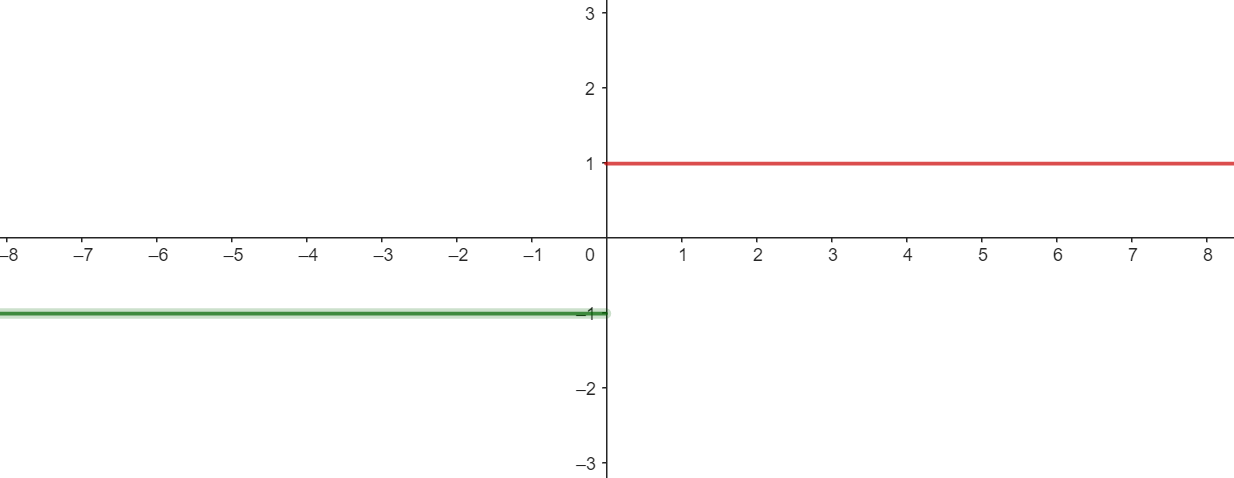
\includegraphics[scale=0.75]{Cours/par morceaux.png}
    \caption{Fonction définie par morceaux    }
    \label{fig:enter-label}
\end{figure}
En 0, la limite à gauche est bien -1 alors que celle à droite est 1. Si l'on approche par chaque côté, la limite est donc différente.
\begin{defi}
    Soit $f\;:\;D(f)\longrightarrow\Rr$ une fonction définie dans un voisinage de $+\infty$.
    On dit que $f$ admet pour limite le nombre $l\in\Rr$ lorsque $x$ tend vers $+\infty$ (ou encore que $l$ est la limite de $f$ en $+\infty$) si
     \[
    \forall \varepsilon>0,\exists M>0 \quad\text{tel que}
    \]
    \[
    x\in D(f), \;x>M \quad \implies \quad |f(x)-l|<\varepsilon .
    \]
    On écrit alors \[
    \lim_{x\rightarrow +\infty}f(x)=l \quad \text{ou} \quad \lim_{x\rightarrow \infty}f(x)=l \quad \text{ou} \quad f(x)\longrightarrow l \; (x\rightarrow +\infty).
    \]
\end{defi}
On peut alors donner une définition analogue de la limite en $-\infty$ ou la définir simplement comme la limite (si elle existe) de la fonction $f(-x)$ en $+\infty$. On écrit alors \[
\lim_{x\rightarrow -\infty}f(x)=l \quad \text{ou} \quad f(x)\longrightarrow l \; (x\rightarrow -\infty).
\]
\begin{defi}
     Soit $f\;:\;D(f)\longrightarrow\Rr$ une fonction définie dans un voisinage $I$ de $a\in\Rr$. On dit que $f$ tend vers $\pm\infty$ lorsque $x$ tend vers $a$ (ou au point $a$) si pour toute suite $(x_n)_{n \in \Nn } \subset I$ telle que 
     \[
     \lim_{n\rightarrow \infty}x_n=a, \text{on a } \lim_{n\rightarrow \infty}f(x_n)=\pm\infty.
     \]
     On écrit alors \[
     \lim_{x\rightarrow a }f(x)=\pm\infty \quad \text{ou} \quad f(x)\longrightarrow\pm\infty \; (x\rightarrow a).
     \]
\end{defi}

On définit de manière analogue les limites infinies à gauche et à droite.

\begin{proposition}
    Soit $f$ et $g$ deux fonctions définie au voisinage de $a\in \Rr$ telles que \[
    \lim_{x\rightarrow a }f(x)=l_1 \quad \text{et} \quad \lim_{x\rightarrow a }g(x)=l_2.
    \]
    On a alors les règles de calcul suivantes:
    \begin{enumerate}
        \item \[
        \lim_{x\rightarrow a }(\alpha f(x) +\beta g(x))=\alpha l_1+\beta l_2, \quad\forall\alpha,\beta\in\Rr .
        \]
        \item \[
        \lim_{x\rightarrow a }f(x)g(x)=l_1l_2.
        \]
        \item $$
        \lim_{x\rightarrow a }f(x)/g(x)=l_1/l_2 $$
        S'il existe un voisinage de $a$ sur lequel $g$ ne s'annule pas et si $l_2\neq 0$.
        
    \end{enumerate}
\end{proposition}
\begin{proposition}
    Soit $f$ une fonction définie au voisinage de $b\in\Rr$ et $g$ définie au voisinage de $a\in\Rr$ telles que $g\neq b$ dans un voisinage pointé de $a$, et 
    \[
    \lim_{x\rightarrow a}g(x)=b, \quad \lim_{y\rightarrow b}f(y)=l.
    \]
    Alors
    \[
    \lim_{x\rightarrow a}f(g(x))=l.
    \]
\end{proposition}

\subsection{Continuité des fonctions}
\begin{defi}
    Soit $f\;:\;D(f)\longrightarrow\Rr$ une fonction définie dans un voisinage de $a \in D(f)$. 
    On dit que $f$ est continue si l'une des deux conditions équivalentes suivantes est satisfaite:
    \begin{enumerate}
        \item \[\lim_{x\rightarrow a}f(x)=f(a).\]
        \item $\forall \varepsilon>0, \exists \delta>0$ tel que $
        0\leq |x-a|<\delta \quad \implies \quad |f(x)-f(a)|<\varepsilon$.
    \end{enumerate}
\end{defi}
\begin{defi}
    Soit  $f\;:\;D(f)\longrightarrow\Rr$ une fonction définie dans un voisinage à gauche de $a \in D(f)$. On dit que f est continue à gauche en $a$ si $limf(x)=f(a)\;(x\rightarrow a^{\_})$.
\\
    On donne une définition analogue de la continuité à droite et on montre aisément que f est continue en $a$ si et seulement si f est continue à gauche et à droite.
\end{defi}
\begin{defi}
    On dit que  $f\;:\;D(f)\longrightarrow\Rr$ est continue sur $(a,b)\subset D(f)$ si $f$ est continue en tout point $x\in(a,b)$.
\\
    On dit que f est continue sur $[a,b]\subset D(f)$ si $f$ est continue sur $(a,b)$ et si $f$ est continue à droite en $a$ et à gauche en $b$.
\\
    Finalement on dit que $f$ est continue si $f$ est continue sur $D(f)$.
\end{defi}

\begin{proposition}
    Soit  $f\;:\;D(f)\longrightarrow\Rr$  et $g\;:\;D(g)\longrightarrow\Rr$ deux fonctions continues.
    Alors si $I\subset D(f) \cap D(g),$ on a que :
    \begin{enumerate}
        \item $\alpha f+\beta g$ est continue sur $I$, $\forall \alpha, \beta \in\Rr$.
        \item $fg$ est continue sur $I$.
        \item $f/g$ est continue sur $I\setminus\{x\in D(f)\cap D(g); \;g(x)=0\}$
        \item Si $g$ est continue en $a\in D(g)$ et $f$ est continue en $b=g(a)\in D(f)$, alors $f\circ g$ est continue en $a\in D(f\circ g)$.
    \end{enumerate}
\end{proposition}
\begin{proposition}
    Une fonction $f\;:\;D(f)\longrightarrow\Rr$ n'est pas continue en $a\in\Rr$ si au moins l'un des trios conditions suivantes n'est pas vérifiée:
    \begin{enumerate}
        \item $a\in D(f)$
        \item  Les deux limites $\lim f(x)\; (x\rightarrow a^{\pm})$ existent (dans $\Rr$) et sont égales.
        \item \[
        \lim_{x\rightarrow a}f(x)=f(a).
        \]
    \end{enumerate}
\end{proposition}
Si l'une des deux dernières conditions n'est pas vérifiée, on dit que f est discontinue en $a$. Si $f$ est discontinue en $a$ mais que les deux limites à gauche et à droite existent, on dit que $a$ est un point de discontinuité de première espèce. Si au moins l'une des deux limites (gauche ou droite) est infinie ou n'existe pas, on dit que a est un point de discontinuité de deuxième espèce (ou discontinuité essentielle) de $f$. Si $a\not\in D(f)$ mais que les limites à droite et à gauche existent et sont finies, on parle de discontinuité apparente et on étend la fonction par continuité.

\begin{defi}
    Soit $f\;:\;D(f)\longrightarrow\Rr$ une fonction continue et $a\not\in D(f)$.
    Alors, si la limite $\lim f(x) \; (x\rightarrow a)$ existe, on définit le prolongement par continuité de $f$ par \[
    \hat{f} \;:\; D(f)\cup \{a\} \longrightarrow\Rr, \quad \hat{f}(x)=
     \left \{
   \begin{array}{c l}
      f(x) & x\in D(f)\\
      \lim_{x\rightarrow a}f(x) & x=a. 
   \end{array}
   \right .
    \]
\end{defi}
Si un tel prolongement existe, il est unique et, par définition, continu. Dans le cas où le domaine de définition est de la forme $(a,b]$ (resp. $[b,a)$), remplacer la limite dans la définition ci-dessus par une limite à droite (resp. à gauche).

Les fonctions sont un outil de prédilection en analyse et meneront à plusieurs outils dont les fameuses intégrales. Vous vous en doutez, bien plus de notions seront vues dans vos cours d'analyse avancée que celles présentées ici. Cependant, bien se souvenir des bases, soit les suites et la définition de continuité à partir des suites, permet de comprendre bien des concepts. 
\end{document}